% !TeX root = main.tex
% !TeX spellcheck = it_IT
\frontmatter
\setcounter{page}{1}
\pagenumbering{Roman}
\tableofcontents
\chapter{Introduzione}
Il nome di Paul Bley non è presente nella memoria collettiva come quello di altri pianisti coevi come Chick Corea o Cecil Taylor.\par
 È un artista la cui vasta discografia si configura come un corpus di pacate riflessioni in ambito jazzistico rispetto ai concetti di tonalità, di tempo, di improvvisazione. Si tratta di una figura cardine nel tentativo di contestualizzare il pianoforte jazz moderno, un ponte poco percorso che collega Ornette Coleman e Keith Jarrett, il free jazz e la musica da camera.\par
 Attraverso le sue collaborazioni con nomi quali Carla Bley, Paul Motian, Steve Swallow, Jimmy Giuffre e Charlie Haden ha attraversato la storia del jazz moderno senza mai smettere di cercare un proprio suono, mai contento di aderire senza precorrere. Maestro dell'\textit{understatement} con un piede nel blues e l'altro nel minimalismo, fautore di una rivoluzione silenziosa che operava dall'interno del linguaggio pianistico e che tutt'oggi, nonostante le ramificazioni delle influenze, sceglie di continuare a non urlare.\par
Nell'introdurre questa breve discussione ringrazio il mio insegnante Nico Morelli per il prezioso insegnamento e il sostegno offerti durante il percorso presso il Conservatorio. Il suo aiuto mi è sempre stato fondamentale per capire le intricate implicazioni dello strumento del pianoforte e per introdurmi, quasi da neofita, alla pratica dell'improvvisazione e della musica jazz. Ringrazio anche gli altri insegnanti che mi hanno aiutato durante il percorso, Maria Luisa Pacciani per le inestimabili indicazioni tecniche e Claudio Vignali per le nuove prospettive sul pianismo jazz. Ringrazio inoltre Alessandro e Lorenzo per la disponibilità e per l'impegno che sono stati per me fondamentali nella preparazione del repertorio della prova finale. Ringrazio infine la mia famiglia per il sostegno durante questo percorso, senza il quale non potrei in alcun modo essere qui.
\mainmatter
\setcounter{page}{1}
\pagenumbering{arabic}
\pagestyle{fancy}
\makeatletter
\let\ps@plain\ps@fancy
\makeatother
\chapter{Cenni biografici}
\section{Montreal: l'infanzia e gli inizi}
Paul Bley nacque a Montreal, in Quebec, il 10 Novembre 1932. I genitori adottivi furono Betty Marcovitch, emigrata rumena di modeste origini, e il facoltoso imprenditore tessile Joe Bley\footcite[10]{stopping}. Paul era in verità figlio biologico di Joe e di una sua dipendente (una donna del Canada francese di nome Lucie): dal momento che Betty non poteva avere figli, Bley fece mettere il neonato in orfanotrofio per convincere poi la moglie, ignara della situazione, ad adottarlo; la madre biologica di Paul venne poi assunta come balia dalla famiglia. Lo stesso Paul non sarebbe venuto a conoscenza di questo fatto fino a molti anni dopo, nel 1992\footcite[13]{stopping}. La madre adottiva, in ogni caso, crebbe il bambino con affetto e cura, decidendo di impartirgli un'educazione musicale e di fargli frequentare la scuola della comunità ebraica di Montreal.\par
La rivelazione del fatto di essere stato adottato (nonostante entrambi i genitori biologici fossero in realtà presenti nel suo nucleo familiare) fu un evento traumatico per il bambino, tanto più che allo stress causato dalla situazione si aggiunse quello provocato dal divorzio dei genitori nel 1939. Il giovane Paul, per far fronte alla mancanza di un senso di appartenenza, trovò così rifugio nella musica e non a caso il pianista ricorda come in quegli anni (anche grazie al suo insegnante August Dècarie) maturò in lui la decisione di diventare un musicista professionista\footcite[15]{stopping}. Sempre in quel periodo Paul ebbe il suo primo contatto con il concetto di improvvisazione:
\begin{fquote}
	Oltre alla scuola, stavo iniziando a studiare per il mio Bar Mitzvah per il quale avrei dovuto cantare un testo in ebraico. Quando chiesi al mio rabbino ``Come fa la melodia?'' egli rispose ``Inventala sul momento\footnote{\cite[16]{stopping}. Le traduzioni dall'inglese di questo (e altri) documenti in questo elaborato sono proprie.}''.
\end{fquote}
Giovanissimo, Bley trova impiego come pianista di varietà al locale della Young Men's Hebrew Association dove venne in contatto con le strutture e le sonorità della musica popolare. Viene in seguito assoldato da altri locali in cui spesso è chiamato a suonare anche con musicisti molto più anziani di lui.
A quattordici anni forma il suo primo gruppo, i \textit{Buzzy Bley}: l'esperienza gli permette di iniziare a farsi conoscere a Montreal e di sviluppare la capacità di gestire, economicamente ed artisticamente, un gruppo di musicisti. \\
Il contatto con il jazz avvenne con la \textit{tramp band} di Al Cowan\footnote{Al Cowan (asse da bucato), B.T. Lundy (sax tenore), Buddy Jordan (tromba), Walter Bacon (batteria). Le \textit{tramp band} erano complessi da intrattenimento che suonavano spesso strumenti bizzari quali, per l'appunto, l'asse da bucato.}, alle cui esibizioni Bley spesso assisteva dopo aver finito di suonare nei locali in cui era ingaggiato. Il gruppo spesso invitava il giovane pianista a suonare e Bley ricorda le dinamiche di apprendimento che venivano a formarsi in quei contesti, tra nottate in locali frequentati da giocatori d'azzardo e prostitute.\par
Nel 1948 Bley potè assistere a un concerto del pianista suo concittadino Oscar Peterson, che nonostante avesse all'epoca solo ventitrè anni già mostrava i segni di un talento geniale e fuori dalla norma, come già all'epoca riconosciuto da Bley\footcite[20]{stopping}. Peterson, a sua volta, rimase impressionato da Bley tanto da chiedergli, alle porte della sua partenza per gli Stati Uniti nel 1949, di sostituirlo come pianista per finire il suo contratto all'Alberta Lounge con il suo bassista e il suo batterista\footnote{Rispettivamente Ozzie Roberts e Clarence Jones.}. Questa fu solo una delle prime fortuite occasioni che, peculiarmente, sarebbero state una costante della vita di Bley. Egli, a suo merito, seppe sempre sfruttarle in maniera congrua.\\
Suonando allo Chalet Hotel Bley venne in contatto con la cantante newyorkese Nina Grey, che lo spinse e lo supportò insieme alla madre Betty nel seguire il proprio sogno di trasferirsi a New York per frequentare la Juilliard School per la musica e le arti a Manhattan. \par
\section{New York e la Juilliard: le prime esperienze}
Nel 1950 Bley si trasferì dunque a New York, dove poté immergersi nella florida scena jazzistica dell'epoca ascoltando le esibizioni di nomi di primissimo rilievo come Charlie Parker, Max Roach, Miles Davis ma anche Lennie Tristano, Lee Konitz e Billy Bauer.\\
Alla Juilliard Bley riceve un'educazione di impostazione moderna, soprattutto in ambito compositivo\footcite[23]{stopping}. Questi anni formativi lasciarono un'impronta profonda sulla sua concezione di tempo, tonalità e soprattutto sul rifiuto della dicotomia, tipica del jazz di quegli anni, di compositore-esecutore.
\begin{fquote}
	Il grande mistero non era se sarebbe arrivata la musica atonale, ma bensì \textit{perchè non fosse ancora arrivata}. [...] A questo riguardo la musica classica ci aveva portati fuori strada, poiché ci aveva spinti a credere che questa svolta sarebbe stata compiuta dai compositori. Nel jazz [...] un compositore è semplicemente qualcuno che non sa suonare in tempo reale.\footcite[24]{stopping}
\end{fquote}
L'atonalità e l'avanguardia, anche attraverso gli insegnamenti del compositore canadese Henry Brant\footcite[23]{stopping} esercitò da subito il proprio fascino su Bley così come su altri musicisti della scuola (come Gil Evans, George Russell e Johnny Carisi che il pianista ebbe modo di conoscere). Alla Juilliard Bley si unì alla \textit{New Jazz Society}, che si riuniva al Downbeat Club dove erano soliti suonare Parker e Charles Mingus il quale, in particolare, fece la conoscenza di Bley proprio in quel contesto.\\
Durante questo periodo, chiaramente, Bley non si fece mancare numerosi ingaggi sopratutto a Brooklyn e a Long Island\footcite[47]{cappelletti} dove cementò la sua familiarità con figure quali il già citato Parker, Jackie McLean e Donald Byrd; grazie al suo manager Monte Kay suonò inoltre per diversi mesi con Lester Young\footcite[47]{cappelletti}.\par
Nonostante la fruttuosa permanenza a New York Bley non abbandonò completamente Montreal, dividendo la propria vita tra le due città negli anni tra il 1950 e il 1953. Nella città canadese Bley si organizzò insieme ad altri due pianisti suoi concittadini, Keith White e Art Roberts, per dare forma al Jazz Workshop. Lo scopo dell'associazione era quello di creare un ambiente di sperimentazione e sviluppo e allo stesso tempo quello di iniettare nuova vita nella scena di Montreal chiamando illustri ospiti da oltre il confine. Si trattò di un'altra azione ``imprenditoriale'' da parte di Bley che durante la sua vita dimostrò sempre una certa inclinazione verso gli aspetti più gestionali della vita del musicista. Tra gli ospiti statunitensi ospitati dal Workshop ci furono Chuck Wayne, Sonny Rollins, Jackie McLean, Art Taylor e, nel 1953, perfino Charlie Parker. Il successo riscosso dell'associazione attirò l'attenzione della televisione canadese CBC che ne trasmise in diretta diversi concerti, compreso quello in cui prese parte Parker\footnote{Queste registrazioni sono disponibili nel disco \textbf{Charlie Parker - \textit{Montreal 1953}} [Uptown Records 1993]. Questo album, nelle tracce 9, 10, 11 e 12 contiene la prima registrazione del pianoforte di Bley, con Neil Michaud (basso), Ted Paskert (batteria), Dick Garcia (chitarra) e Brew Moore (sax tenore).}. Bley ricorda la differenza tra la scena di Montreal, in cui i musicisti esperti si facevano paternalmente carico dell'istruzione di quelli più giovani, e quella di New York. ``\textit{I giovani musicisti non si consideravano discepoli e la conoscenza dei musicisti più anziani era disponibile solo in vendita. Se volevo che Charlie Parker suonasse con me dovevo ingaggiarlo}\footcite[31]{stopping}''. A riprova della sua inclinazione manageriale, Bley si fece carico di scortare un Parker stralunato e ormai in preda alla propria tossicodipendenza da New York a Montreal (temendo che si sarebbe perso in aeroporto e sarebbe finito in Alaska). Parker deve aver apprezzato il pianismo di Bley, poichè lo richiamò in seguito per un ingaggio a Brooklyn\footcite[34]{stopping}. L'esperienza segnò profondamente Bley, che rimase colpito da come il sassofonista riuscisse a ``\textit{prevedere ciò che stava arrivando e pensare sempre in anticipo}''\footcite[35]{stopping}.\par
Nel 1953 Charles Mingues chiamò Bley per una registrazione come direttore d'orchestra\footnote{Composta da Janet Thurlow (voce), Charles Mingus (basso), Kenny Clarke (batteria), John Lewis (pianoforte), Ernie Royal (tromba), Danny Bank (sax baritono), Willy Dennis (trombone), Eddie Caine (sax contralto e flauto), Teo Macero (sax tenore) e Jackson Wiley (violoncello).} per alcuni pezzi nel contesto di un progetto della neonata etichetta discografica di proprietà di Mingus, la Debut Records. A questo ingaggio Mingus aggiunse un'ulteriore registrazione in trio con Art Blakey. Quest'ultima prova, pubblicata come \textbf{Paul Bley - \textit{Introducing Paul Bley}} [Debut 1954] nonostante la \textit{line-up} di primo livello appare piuttosto sbiadita e priva di carica, tanto che Cappelletti insinua che fosse stata proposta da Mingus più come forma di ringraziamento per il lavoro di direzione di orchestra che come dichiarazione di fiducia nelle doti pianistiche di Bley\footcite[49]{cappelletti}.\par
\section{L'esperienza free: Coleman, Russell, Giuffre, Rollins}
Nel 1955 Bley ricevette un ingaggio da Chet Baker per un tour di esibizioni ad Hollywood; nel 1956 venne chiamato dalla cantante Dakota Staton per poi iniziare un tour del Midwest americano con Lennie McBrown (batteria) e Hal Gaylor (basso a cinque corde)\footcite[49]{stopping}. Nello stesso anno al Birdland di New York fece la conoscenza di Karen Borg (destinata a diventare nota come Carla Bley e a essere, per un periodo, moglie di Paul), che all'epoca lavorava nel locale come cameriera. \\
In generale quello in California fu un periodo molto intenso per Bley, tanto che nel 1957 ebbe un malore e fu ricoverato per un'emorragia interna causata da un'ulcera duodenale. Bley attribuisce\footcite[54]{stopping} l'episodio al suo continuo stato di irrequietezza, nato con la rivelazione di essere stato adottato, che lo spingeva a trascurare la propria salute fisica e mentale a vantaggio degli impegni lavorativi. In seguito all'episodio Bley sostiene di aver realizzato la maggiore importanza dello stato artistico della musica jazz rispetto alla propria carriera individuale. Dopo il ricovero Bley viene raggiunto a Los Angeles da Karen Borg, con la quale aveva iniziato una relazione da qualche tempo, per poi sposarsi e stabilirsi in California.\par
Nel 1957 ottenne un ingaggio all'Hillcrest Club sul Washington Boulevard a Los Angeles con Gaylor e McBrowne a cui si aggiunse Dave Pike (vibrafono). Parallelamente approfondisce inoltre la strada dell'improvvisazione libera in duo con il trombettista Herbie Spanier\footcite[58]{stopping}. Dovendo sostituire Gaylor, che aveva deciso di trasferirsi a est, McBrowne presentò a Bley il contrabbassista Charlie Haden. Ricorda Bley: ``\textit{Charlie arrivò scalzo. Non solo non aveva le scarpe, ma anche la sua scelta di note lasciava abbastanza a desiderare. Il suo modo di tenere il tempo era impeccabile [...] sarebbe stato facile trovare un altro bassista che suonava le note corrette ma avrei dovuto essere molto fortunato per trovare un altro bassista con un senso del tempo così}\footcite[62]{stopping}''. Poco dopo anche McBrowne tornò ad est sotto ingaggio di Horace Silver e fu così sostituito da Billy Higgins a completare la sezione ritmica. Una sera quest'ultimo propose a Bley di conoscere un trombettista e un sassofonista con cui lui e Haden stavano lavorando: si trattava, ovviamente, di Don Cherry e di Ornette Coleman.
\begin{fquote}
	Il fatto che fosse successo in una notte qualunque di un ingaggio di due anni fu una sorpresa, ma non servì più di un secondo per capire che quello era l'anello mancante tra suonare in maniera totalmente \textit{free}, senza vincoli di sorta, e suonare \textit{bebop} con cambi di accordi e tempo stabile.\footcite[64]{stopping}
\end{fquote}
Bley iniziò così la sua esperienza con Coleman (che gli sarebbe costata il posto di lavoro all'Hillcrest\footcite[51]{cappelletti}) esplorando diverse concezioni di tempo, struttura (Bley aveva sempre mal sopportato la ridondanza di sezioni A e B nella forma canzone tradizionale) e armonia. Parte di queste performance, che Bley registrava su nastro, sono documentate dai dischi \textbf{\textit{The Fabulous Paul Bley Quintet}} [America Records 1970] e \textbf{\textit{Ornette Classics 1}} [Improvising Artists 1977]. \par
Dopo un breve ingaggio con Scott LaFaro (basso), Bobby Hutcherson (vibrafono) e Larance Marable (batteria), Carla e Paul tornarono a New York nel 1959 dove la fama di Coleman precedeva il nome del pianista\footcite[70]{stopping}. Nel 1960 venne chiamato da George Russell, che aveva avuto modo di ascoltare Bley qualche tempo addietro alla Lenox School of Jazz, per un progetto di un pezzo per due pianoforti e Orchestra per la Decca Records in quello che sarebbe poi uscito con il titolo di \textit{\textbf{Jazz in the Space Age}} [Decca 1960]. Compositore affermato, Russell aveva concepito una teoria armonica basata sulla \textit{gravità tonale}\footcite[3]{russell} e su un'organizzazione tonale incentrata sul cromatismo interpretato come naturale estensione della serie armonica\footcite[12]{russell}, prospettiva che senza dubbio ben si complementava con la fuga dalla tonalità (benchè Russell di fatto proponesse un \textit{rafforzamento} parossistico del concetto di tonalità) che caratterizzava la musica di Coleman.\\
L'altro pianista chiamato a realizzare il progetto era Bill Evans, in quegli anni all'apice della sua popolarità dopo le registrazioni di \textit{\textbf{A Kind Of Blue}} [Columbia 1959]. Bley racconta stupito di come questi si era inaspettatamente rivelato in sintonia con le sue idee di sperimentazione e atonalità, tanto da preoccuparsi che Evans potesse rubargli la scena e lasciarlo senza lavoro. Con suo grande sollievo, però, Bley racconta che dopo le registrazioni andò ad ascoltare il trio di Evans al Village Vanguard per scoprire che il pianista, al di là dell'esperienza con Russell, non sembrava interessato ad allontanarsi da quella che era la sua zona di comfort\footcite[75]{stopping}.\par
In questi anni Bley conobbe il bassista Steve Swallow, con il quale si ritrovò a suonare in diverse occasioni in duo. Contestualmente, fu anche chiamato dal chitarrista Jim Hall per sostituirlo in un trio con il clarinettista e sassofonista Jimmy Giuffre e il bassista Ralph Peña. Giuffre, così come Russell, aveva avuto modo di ascoltare Bley alla Lenox School of Jazz rimanendo intrigato dallo stile anticonvenzionale del pianista. In seguito all'abbandono di Peña, Bley convinse Giuffre ad assumere (a scatola chiusa) Swallow come bassista. Soddisfatto dal suono del trio, Giuffre portò il gruppo per una (sfortunata\footcite[77]{stopping}) tournee in Europa nel 1961. Dello stesso anno sono i due dischi che documentano questa iterazione dei \textit{Jimmy Giuffre 3}, cioè \textit{\textbf{Thesis}} [Verve 1961] e \textit{\textbf{Fusion}} [Verve 1961], in cui già si nota una prevalenza di brani scritti da Carla Bley (tendenza, questa, che non avrebbe mai abbandonato Paul nemmeno dopo la separazione). Un ulteriore album, \textit{\textbf{Free Fall}} [Columbia 1963] portò a un livello ancora più avanzato la proposta di improvvisazione collettiva di Giuffre. Là dove nei primi due dischi si avvertiva ancora una forma compositiva, in \textit{Free Fall} si assiste a uno sgretolamento di quest'ultima in favore di una libertà espressiva quasi totale. Si una forma di free jazz fortemente alternativa a quella \textit{mainstream} di quegli anni e anche per questo non salutata da un particolare successo commerciale, tanto che il gruppo si sciolse nel 1963 dopo una serata il cui magro incasso era ammontato a trentacinque centesimi a testa\footcite{hamilton}.\par
In seguito a una proposta di Herbie Hancock nel 1963 Bley fu ingaggiato da Sonny Rollins insieme a Henry Grimes (basso) e Roy McCurdy (batteria) per una serie di concerti, un tour in Giappone e Stati Uniti e un disco per la RCA con Coleman Hawkins, \textit{\textbf{Sonny meets Hawk!}} [RCA Victor 1963]. A differenza delle esperienze precedenti, il repertorio di Rollins era costituito principalmente da \textit{standard} seppur suonati con grande libertà armonica e strutturale. Questa occasione diede a Bley l'opportunità di misurarsi con un ulteriore approccio al linguaggio \textit{free}: il legame tra gli \textit{standard} e il pianista sarebbe continuato anche in seguito, fino alla fine della sua carriera.
\section{La maturità artistica: il trio, l'incontro con l'elettronica e il solo}
Nel 1964 Bley fu assoldato dal bassista Gary Peacock per una doppia serata: il primo concerto insieme a John Gilmore (sax tenore) e a Paul Motian (batteria) e il secondo con Albert Ayler (sax tenore) e Sunny Murray (batteria)\footcite[89]{stopping}. L'esperienza con Murray, primo batterista \textit{free} con cui Bley avesse mai avuto a che fare, fu allo stesso tempo rivelatrice e traumatica, tanto che Bley dovette chiedere a Carla di riscrivere i propri brani affinché si adattassero meglio allo stile del batterista. Non a caso, Bley avrebbe poi nella propria carriera prediletto lo stile più controllato di Motian. Gli sforzi di questa fase della carriera di Bley sono documentati nei dischi \textit{\textbf{Turning point}} [Improvising Artists 1975] con il primo quartetto e \textit{\textbf{Barrage}} [ESP-disk 1964] con Marshall Allen (sax contralto), Dewey Johnson (tromba), Eddie Gomez (basso) e Milford Graves (batteria).\par
Nello stesso anno Bley fu invitato dal trombettista Bill Dixon a prendere parte agli incontri dell'associazione Jazz Composer Guild. L'idea dell'associazione era quella di formare una sorta di sindacato per opporsi alle pratiche scorrette dei \textit{leader} delle formazioni e delle etichette discografiche. Seppur riluttante all'inizio\footnote{``L'incontro era un manipolo di anime in pena. Alla faccia della terapia di gruppo...'' \cite{stopping}, p. 91.}, Bley si ritrovò insieme al trombonista Roswell Rudd alla direzione dell'associazione in seguito alla defezione di Dixon. Durante questa nuova esperienza da organizzatore e gestore Bley riuscì a produrre diversi concerti e a guadagnare nuovi membri (tra tutti, il pianista Cecil Taylor). Il nuovo successo dell'organizzazione permetteva anche a musicisti meno noti, come a quel tempo il quintetto di Carla Bley con il trombettista (e futuro marito di Carla) Mike Mantler, di godere di un'utile visibilità. In quegli anni Carla Bley, sotto consiglio di Paul, potè utilizzare i leader delle formazioni nella Jazz Composer's Guild per formare la Jazz Composer's Orchestra Association insieme a Mantler. Bley ricorda che l'idea fu ``così buona da costarmi una moglie''\footcite[95]{stopping}, dato che nel 1965 Paul e Carla divorziarono.\par
In seguito alla sofferta separazione, iniziò per Bley un approfondimento della forma e delle potenzialità della formazione in trio\footcite[98]{stopping}. Il primo passo in questa direzione, \textit{\textbf{Closer}} [ESP-disk 1965] con il già citato Steve Swallow e Barry Altcschul (batteria). Per il disco Bley adottò, in controtendenza con il \textit{free} dell'epoca, la scelta di limitare la lunghezza dei soli ottenendo così una \textit{tracklist} più folta e con una maggiore varietà di temi e atmosfere\footnote{Bley, tra i cui difetti non si può certo annoverare la modestia, equipara \textit{Closer} ai dischi di Albert Ayler a livello di importanza storica per il jazz. \cite[100]{stopping}.}. Grazie al sostegno della ESP, Bley potè portare il proprio trio (con Kent Carter al basso) in Europa per un tour nello stesso anno).\par
Nel 1966 Bley iniziò una relazione, e in seguito matrimonio, con la compositrice e pioniera della musica elettronica Annette Peacock (ex moglie del bassista Gary Peacock). Come con Carla Bley, Peacock sarebbe divenuta una presenza molto importante nella vita personale e artistica di Bley, che avrebbe suonato composizioni delle sue prime due mogli per il resto della propria carriera. Nello stesso periodo Bley e Peacock si recarono in Europa insieme ad altri nomi della scena (tra cui Steve Lacy, Altschul e Carla Bley).\\
Paradossalmente, in Europa Bley trovò sempre un'accoglienza migliore rispetto agli stati uniti. Dopo un festival a Madrid con Altschul e Mark Levinson (basso), Bley fu invitato a Bologna da cui poi nacque un tour di sei mesi per l'Italia\footcite[102]{stopping}. Come altre personalità quali Steve Lacy e Don Cherry, Bley e Peacock risiedettero per qualche a tempo a Roma sotto l'egida del produttore RCA Alberto Alberti\footcite[104]{stopping}. Dall'esperienza nacque il disco in trio \textit{\textbf{Ramblin'}} [RCA Italia 1966]. Dopo altre esperienze sui palchi europei nello stesso anno (con cinque dischi dal vivo e in studio rilasciati durante il periodo), Bley ricorda come nella formazione in trio aveva finalmente trovato un campo espressivo in cui sentirsi libero:
\begin{fquote}
	Suonavo tutto io. Niente fiati. Finalmente potevo mettere in pratica le \text{mie} idee di free jazz. [...] Questo trio poteva aprire le finestre e dare ossigeno a tradizioni che avevano raggiunto un blocco.\footcite[106]{stopping}
\end{fquote}
Nel 1969 l'attenzione di Bley venne catturata dai sintetizzatori con tastiera (che iniziavano in quegli anni ad apparire sul mercato). Dopo aver convinto Robert Moog in persona a procurargli uno dei pochi esemplari di sintetizzatore semi-modulare in produzione dall'azienda\footcite[110]{stopping}, Bley e Peacock iniziarono ad esplorare le potenzialità dello strumento. I due iniziarono una serie di esibizioni (il \textit{Bley - Peacock synthesizer show} in cui Peacock, tra l'altro, fu pioniera della tecnica della sintesi vocale) anche in Europa. In particolare, Peacock fu notata da David Bowie proprio in virtù delle sue sperimentazioni vocali. I risultati di queste esplorazioni sono negli album \textbf{\textit{Improvisie}} [America 1971], \textit{\textbf{Dual Unity}} [Freedom Records 1972] e il primo album solista di Peacock \textit{\textbf{I am the one}} [RCA 1972]. La fine di questo periodo marcò anche la fine della relazione tra Bley e Peacock.\par
Nello stesso anno il discografico Manfred Eicher, della casa tedesca ECM, propose a Bley un disco in pianoforte solo per il catalogo dedicato\footcite[119]{stopping} (in cui già facevano novero Chick Corea e Keith Jarrett). Nonostante Bley non avesse mai prodotto nessun lavoro nella forma del piano solo, il risultante \textit{\textbf{Open, to Love}} è considerato uno dei punti più significativi della carriera del pianista\footcite[75]{cappelletti}. Il disco, contente brani di Carla Bley, di Peacock e dello stesso Paul, offre una summa della proposta pianistica dell'artista condensata in una forma ancora più diretta del trio.\par
Durante una permanenza a Copenhagen dove Bley registrò con il bassista autoctono Niels-Henning Ørsted Pedersen il disco \textit{\textbf{Paul Bley/NHØP}} [SteepleChase Records 1973], il pianista conobbe l'artista visuale Carol Goss, che sarebbe diventata la sua terza (e ultima) moglie. Dopo essere scampato a un incendio nella sua abitazione di New York (durante il quale Bley rischiò la vita per salvare il sintetizzatore in cui a suo dire non era nemmeno più interessato\footcite[120]{stopping}), Bley e Gross fondarono la compagnia di registrazioni audio-video Improvising Artists Inc. la cui idea era quella di invitare piccole ensemble di musicisti di estrazione trasversale al \textit{free} come Sun Ra, Sam Rivers o Lee Konitz. Curiosamente, la prima registrazione esistente degli allora giovanissimi Jaco Pastorius e Pat Metheny appartiene proprio alla neonata etichetta di Bley (il disco \textit{\textbf{Jaco}} [Improvising Artists 1974]). L'etichetta fu anche promotrice dei primi pioneristici esperimenti di perfomance audio-visiva in ambito jazz ad opera di Goss: n particolare nel 1977 Sun Ra e Bley presero parte a questa performance ibrida di musisciti e sintetizzatori video\footcite[129]{stopping}. In quel periodo, il successo dei dischi più orientati a un sound elettrico (non solo della sua etichetta, ma in generale per le direzioni intraprese da pianisti come Joe Zawinul, Herbie Hancock e Chick Corea) spinse Bley a scegliere di differenziarsi focalizzando i suoi sforzi sul pianoforte acustico\footcite[127]{stopping}. \par
Dopo sette anni di attività discografica, Bley e Goss decisero di chiudere la società per concentrarsi sulla propria produzione artistica e sul proprio matrimonio\footcite[132]{stopping}.\par
\section{Il tramonto della carriera: tour e insegnamento}
L'esperienza di \textit{business} maturata negli anni e il fitto network di conoscenze tra musicisti di Bley gli permisero, alla soglia degli anni '80, di intraprendere una fitta stagione di concerti e di \textit{reunion.} Tra queste, una sfortunata tournée con Chet Baker nel 1985 (trent'anni dopo la loro prima collaborazione), in cui Bley ebbe l'esperienza di un trombettista ormai non più in condizione di reggere un tour a causa della sua tossicodipendenza\footcite[137]{stopping}. \\
Nel 1989 l'editor del \textit{Jazz Magazine} parigino Phillipe Carles organizzò una riunione del progetto Jimmy Giuffre 3 con Steve Swallow (ora al basso elettrico e marito di Carla Bley) in Europa, dove a differenza degli anni '60 venne ora accolto tra gli onori generali\footcite[137]{stopping}. Dall'esperienza furono prodotti i dischi \textit{\textbf{The Life of a Trio: Saturday}} [Owl Records 1990] e \textit{\textbf{The Life of a Trio: Sunday}} [Owl Records 1990]. \par
È a questo periodo che risale la fase più prolifica, a livello di registrazioni, di Bley: adducendo come causa di questo nuovo desiderio di entrare in sala di registrazione il fatto di aver ridotto al minimo le occasioni di suonare. Questi anni di attività corrispondono anche a un approccio più rilassato e meno competitivo di Bley rispetto alla pratica pianistica e alla scena jazz\footcite[82]{cappelletti}.\par
Nel 1993 Bley ritorna eccezionalmente al sintetizzatore (questa volta, però, digitale) ventidue anni dopo il suo ultimo disco elettronico nel 1971\footcite[148]{stopping}
. Il risultato è \textit{\textbf{Synth-Thesis}} [Postcard Records 1993]. Nello stesso anno, nonostante le proprie reticenze verso l'insegnamento, accetta una sporadica cattedra al Conservatorio del New England a Boston (lo stesso dove Giuffre aveva insegnato per anni). Tra i suoi allievi più illustri figurano la pianista giapponese Satoko Fujii e il compositore israeliano Yitzhak Yedid.\par
Paul Bley morì il 3 gennaio 2016 nella sua casa a Stuart, in Florida, di cause naturali.
\chapter{L'estetica pianistica e improvvisativa}
\section{Farneticando con Ornette}
\begin{fquote}
	Non sono mai stato un amante degli accordi. Ho sempre pensato che un accordo fosse una melodia verticale suonata simultaneamente: se un accordo non poteva essere dissezionato in maniera tale che ogni nota si allineasse a formare una melodia di senso compiuto, non era un buon accordo.\footcite[71]{stopping}
\end{fquote}
Una delle caratteristiche più lampanti dello stile improvvisativo di Bley risiede senza dubbio nel suo approccio, che fonde in uno stile ``polifonico''\footcite[50]{cappelletti} concezioni di natura melodica e armonica. \par
È interessante notare come anche nella prima fase della carriera di Bley, più legata al linguaggio bebop e all'armonia tradizionale, vi fossero già delle caratteristiche tipiche anche dei lavori successivi\footcite[104]{dean}. Ad esempio, nel primo disco di Bley da solista \textit{Introducing Paul Bley} [Debut 1953] con Art Blakey e Charles Mingus, si nota già una spiccata tendenza alla manipolazione armonica. Ad esempio, l'introduzione di \textit{I Can't Get Started} (in figura \ref{fig:cant}) mostra già quello che probabilmente è l'influsso degli insegnamenti di Brant, con una chiara impronta polifonica dell'andamento delle due mani e una scelta di intervalli dal suono scuro e dissonante.
Si tratta ancora, chiaramente, di una sperimentazione piuttosto marginale (e in ogni caso meno avanzata dei risultati che ad esempio Lennie Tristano aveva ottenuto in anni precedenti). \\
Emerge già in ogni caso, come punto di rottura con il linguaggio melodico bebop da cui Bley ancora attinge (e attingerà in seguito) a piene mani, la tendenza a cercare ed ostentare un senso di continuità con lunghe frasi melodiche monoritmiche, spesso anche monofoniche, che si estendono spesso anche oltre la struttura di pertinenza. È interessante, a tal proposito, notare come già in questo album si riscontra la tendenza di Bley all'esporre i temi in maniera minima, senza armonizzazioni o \textit{block chords} di sorta.
\begin{figure}[H]
	\centering
	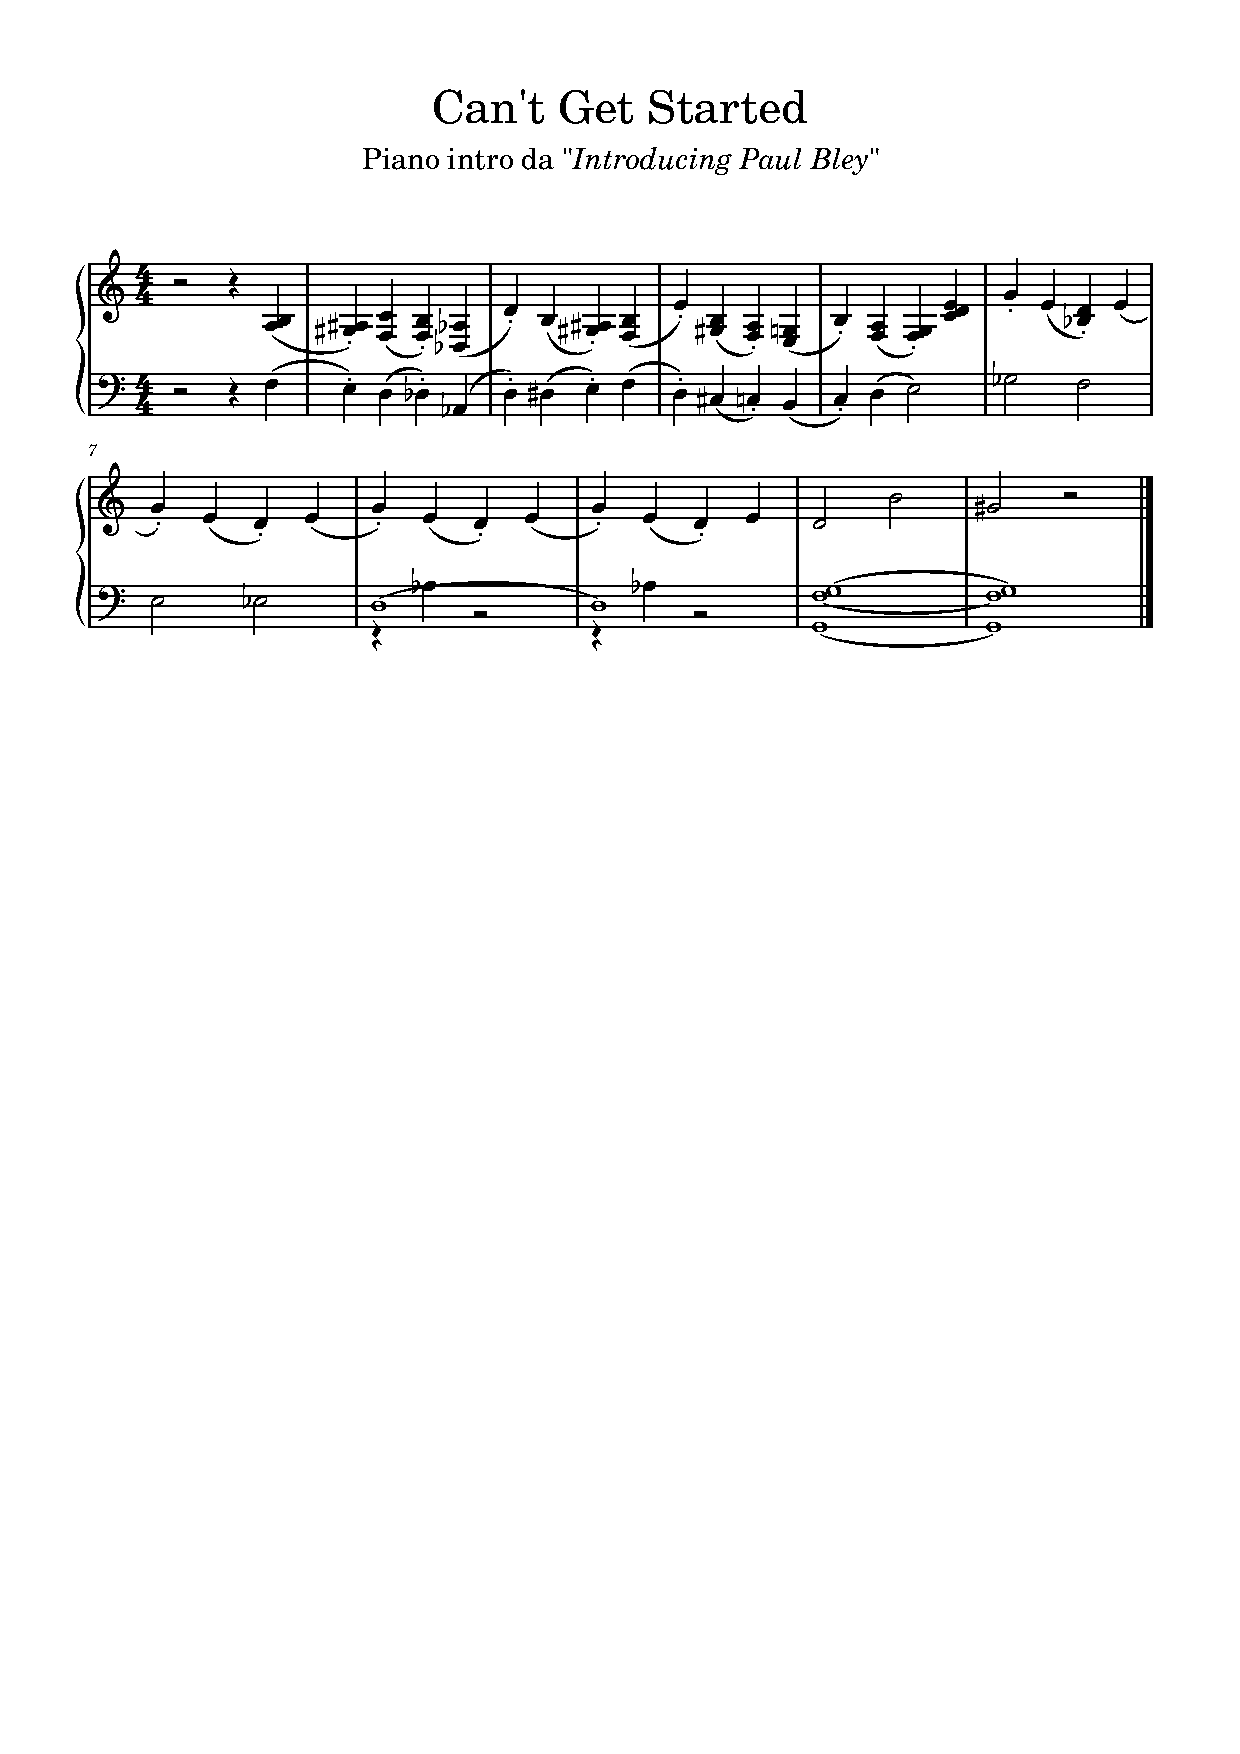
\includegraphics[clip,trim=1cm 18cm 1cm 4.3cm, width=\textwidth]{cantgetintro.pdf}
	\caption{Introduzione di \textit{I can't Get Started} da \textit{Introducing Paul Bley}}
	\label{fig:cant}
\end{figure}
Chiaramente, l'incontro con Coleman può essere visto come la scintilla che porta davvero Bley ad abbracciare il linguaggio free; è bene ricordare, però, che il linguaggio entro cui Bley si muove è sempre prettamente jazz e il cordone ombelicale della continuità con la tradizione non viene mai davvero reciso. L'impiego delle forme bebop come l'abbassamento della quinta o della terza sugli accordi di dominante o i circondamenti delle note accordali è ricorrente e sistemico sia prima che dopo il contatto con Coleman\footcite[26]{meehan}. Bley fa spesso uso delle scale esatonali (come si può sentire in tutte le registrazioni con Jimmy Giuffre nel 1961), delle scale alterate e soprattutto del linguaggio blues.\\
\begin{figure}[h]
	\centering
	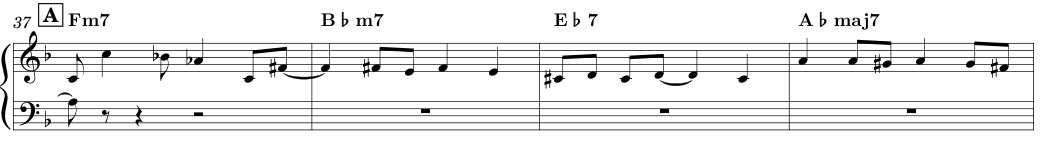
\includegraphics[width=\linewidth]{screenshot001}
	\caption{Esempio di utilizzo di scala esatonale nel solo di \textit{All the things you are} nel disco \textit{Sonny Meets Hawk!}}
	\label{fig:screenshot001}
\end{figure}   
In particolare, vale la pena di approfondire l'evidente ascendente che la musica di Coleman ha evidentemente esercitato per tutta la vita del pianista.
\begin{fquote}
	Ornette ha risolto, con una singola mossa, un problema che era in fase di accumulazione da dieci anni. Ciò consisteva nel capire cosa fare per rendere l'improvvisazione jazz più interessante. Bird era un virtuoso sui cambi armonici e dopo di lui ne sono arrivati a dozzine. Non c'era niente di rimasto da suonare: ciò che avevi era una forma canzone di trentadue battute, una più una meno, che era ormai consunta come base su cui suonare. Quindi, ciò che Ornette fece fu dire che dopo la melodia tu dovevi suonare su solo uno dei centri tonali della melodia. Scriveva i temi deliberatamente in modo tale che non ci fossero trentadue battute di cambi armonici equamente distribuiti. Suonavano come se fossero tonali, ma a un esame più approfondito della composizione le battute erano irregolari e cose così.\footcite[12]{downbeat74}
\end{fquote}
Anche per Coleman, così come per Bley, si può notare il suo vocabolario musicale sia in fin dei conti direttamente mutuato da quello swing, bebop e rhythm \& blues e che l'operazione effettivamente innovativa consista nel nuovo significato dato dalla combinazione di questi motivi tradizionali in nuovi pattern metrici e melodici: l'innovazione non sta quindi nella creazione di un nuovo vocabolario ma bensì nella ridefinizione della sintassi e della grammatica musicale\footcite[109]{cogswell}. Senza alcun dubbio questa tendenza era compatibile con la determinazione di Bley di rimanere, in ogni caso, nell'ambito di un campo comunicativo jazzistico. La già citata continuità nelle frasi di Bley costituisce un altro punto in comune con l'estetica di Coleman, in cui emerge una volontà quasi metodica di mettere in relazione ogni motivo con quello precedente e quello successivo\footcite[115]{cogswell}.\par
In questo senso la continuità melodica di Bley in tutte le fasi della carriera lo ha sempre contraddistinto se messo a confronto con pianisti quali Cecil Taylor, per cui invece vi è il tentativo di scardinare la coerenza non solo del linguaggio pianistico, ma anche della tecnica. In questo senso lo stile solistico di Bley è fortemente melodico non tanto rispetto all'armonia intesa in senso boppistico (che Bley, molto spesso, sceglie di non seguire) quanto più in relazione alla continuità interna del fraseggio. In Bley vi è spesso un fluire ininterrotto di idee melodiche che vengono concatenate, elise e combinate\footcite[20]{meehan}. Armonicamente, le continue escursioni di tonalità di Bley, che però non si incanala mai in una vera e propria bitonalità o politonalità, potrebbero rientrare nel concetto di \textit{pantonalità}\footcite[73]{reti} che in contrasto con l'atonalità propriamente definita, in cui il concetto stesso di tensione e rilascio armonico è effettivamente reso nullo, mostra una continua produzione e rilascio di dissonanze senza una reale soluzione di continuità.\par
Un altro concetto Colemaniano che ha probabilmente esercitato una forte influenza sul pianista è quello di \textit{erasure phrases}, che Bley spiega come ``frasi che erano tonali e ben temperate [alternate a] frasi che invece non lo erano deliberatamente\footcite[67]{stopping}'' con lo scopo di ``cancellare dalla tua memoria ciò che hai appena ascoltato.[...] Non sono lì per dirti qualcosa ma per farti dimenticare. Sono lì per farti sciacquare la bocca\footcite[32]{meehan}''. Ovviamente, per il pianoforte, strumento temperato per eccellenza, era impossibile riprodurre le variazioni microtonali di intonazione che caratterizzavano lo stile di Coleman; a tal proposito Bley sviluppa una metodologia personale per dare l'effetto di \textit{erasure phrase} in diversi punti dei propri soli. Come si può notare nelle trascrizioni dei soli di \textit{Ramblin'} (fig. \ref{fig:ramblin}) e \textit{All The Things You Are}, Bley spesso si trova a suonare passaggi che sono composti da frammenti di materiale tonale ad alta densità di note che, di conseguenza, eludono un centro tonale esatto e offuscano il senso armonico imitando la sensazione di disorientamento data dalle frasi non temperate suonate da Coleman. L'ambiguità riguarda anche l'aspetto ritmico: queste frasi sono spesso costituite da una scarica fitta di note senza una scansione ritmica regolare, con frequenti micro-interruzioni, inciampi, accelerazioni e ritenuti. Sono definibili come \textit{gesti}, piuttosto che vere e proprie melodie con coerenza interna, posti tra due idee melodiche dotate invece di autosufficienza e rilevanza.\par 
A tal proposito appare inevitabile, per Bley, la riflessione sui limiti intrinseci allo strumento del pianoforte quando messo a confronto con la libertà timbrica e di intonazione del sassofono.
\begin{fquote}
	Spendevo tre quarti del tempo facendo accordare Ornette per vedere se sarei riuscito a fargli suonare il la a 440 Hz... Purtroppo io non avevo la stessa flessibilità che aveva lui quando si trattava di suonare un la.\footcite[62]{litweiler}
\end{fquote}
L'interrogazione sui limiti timbrici del pianoforte, unita alla teoria, anch'essa mutuata da Coleman, della mancanza di equivalenza dei toni a diverse ottave (per la quale una stessa nota a ottave differenti non dovrebbe essere considerata, appunto, la ``stessa'' nota\footcite[110]{dean}) avrebbe portato Bley a esplorare i suoni interni del pianoforte (tecnica usata, ad esempio, in \textit{Olhos de Gato} in \textit{\textbf{Alone, again}} [Improvising Artists 1976] in cui la cordiera del pianoforte viene pizzicata o in \textit{Touching 1} da \textit{\textbf{Mr. Joy}} [Mercury 1968] dove Bley opera una sorta di glissato sulle corde individuali). Sempre questa ricerca di nuove possibilità al di là del rigido temperamento del pianoforte sarebbe stata, con tutta probabilità, anche la chiave dell'interessamento agli strumenti elettronici negli anni '70.\par
Bley aveva inoltre sempre mal sopportato la ripetitività della forma canzone\footnote{``{Se ci metti un minuto a suonare una sezione AABA hai già suonato tre sezioni ridondanti nel primo minuto. Tenere questo passo per quindici minuti, con tre sezioni A al minuto, è ridondanza all'estremo}.'' \cite[25]{stopping}} e aveva cercato nella dissoluzione della struttura una risposta a questa esigenza interpretativa, con il risultato che questo approccio rischiava di portare a un vicolo cieco dal momento che ``[suonare] \textit{totalmente free} non ti permetteva necessariamente di continuare [...], fine del concerto''; l'esperienza all'Hillcrest con Coleman fu in questo senso illuminante: 
\begin{fquote}
	suggeriva [una struttura del tipo] ABCDEFGHIJK in cui la ripetizione era un anatema. Non era completamente free perchè completamente free significava una sezione A per sempre in metamorfosi. Era una forma che aveva senso perchè tu finalmente potevi tornare alla musica scritta e il pubblico aveva qualcosa a cui aggrapparsi.\footcite{hamilton}
\end{fquote}
In questo modo si può dire che Coleman avesse offerto un modo di comporre spontaneamente attraverso l'improvvisazione melodie in emergenza da quella originale, generando nuovi pattern basato sulla direzione, velocità o sul materiale melodico dell'originale\footcite[305]{gluck}. La connessione biunivoca tra composizione e improvvisazione è sempre stata cara a Bley\footcite[22]{cappelletti} e non è un caso, in fin dei conti, che egli sia stato uno dei pochi pianisti con cui Coleman abbia mai suonato (oltre a Joachim Kuhn e Geri Allen). Forse il già citato approccio orizzontale all'armonia ben si sposava con la libertà richiesta da Ornette nell'accompagnamento.\par
In particolare, questo sincretismo tra tradizione, innovazione, linguaggio blues e concezione Colemaniana si presenta all'ascoltatore analizzando gli ultimi due \textit{chorus} di solo di piano di \textit{Ramblin'} dall'omonimo album registrato in Italia nel 1966 (in figura \ref{fig:ramblin}). In questo blues dalla forma aperta (che però Bley in questo disco approccia con una maggiore fedeltà alla struttura classica a dodici battute) appare evidente come si passi con relativa disinvoltura da un vocabolario strettamente blues a invece un fraseggio lungo, spezzato e non rispettoso della struttura armonica. \par 
\begin{figure}[h]
	\centering
	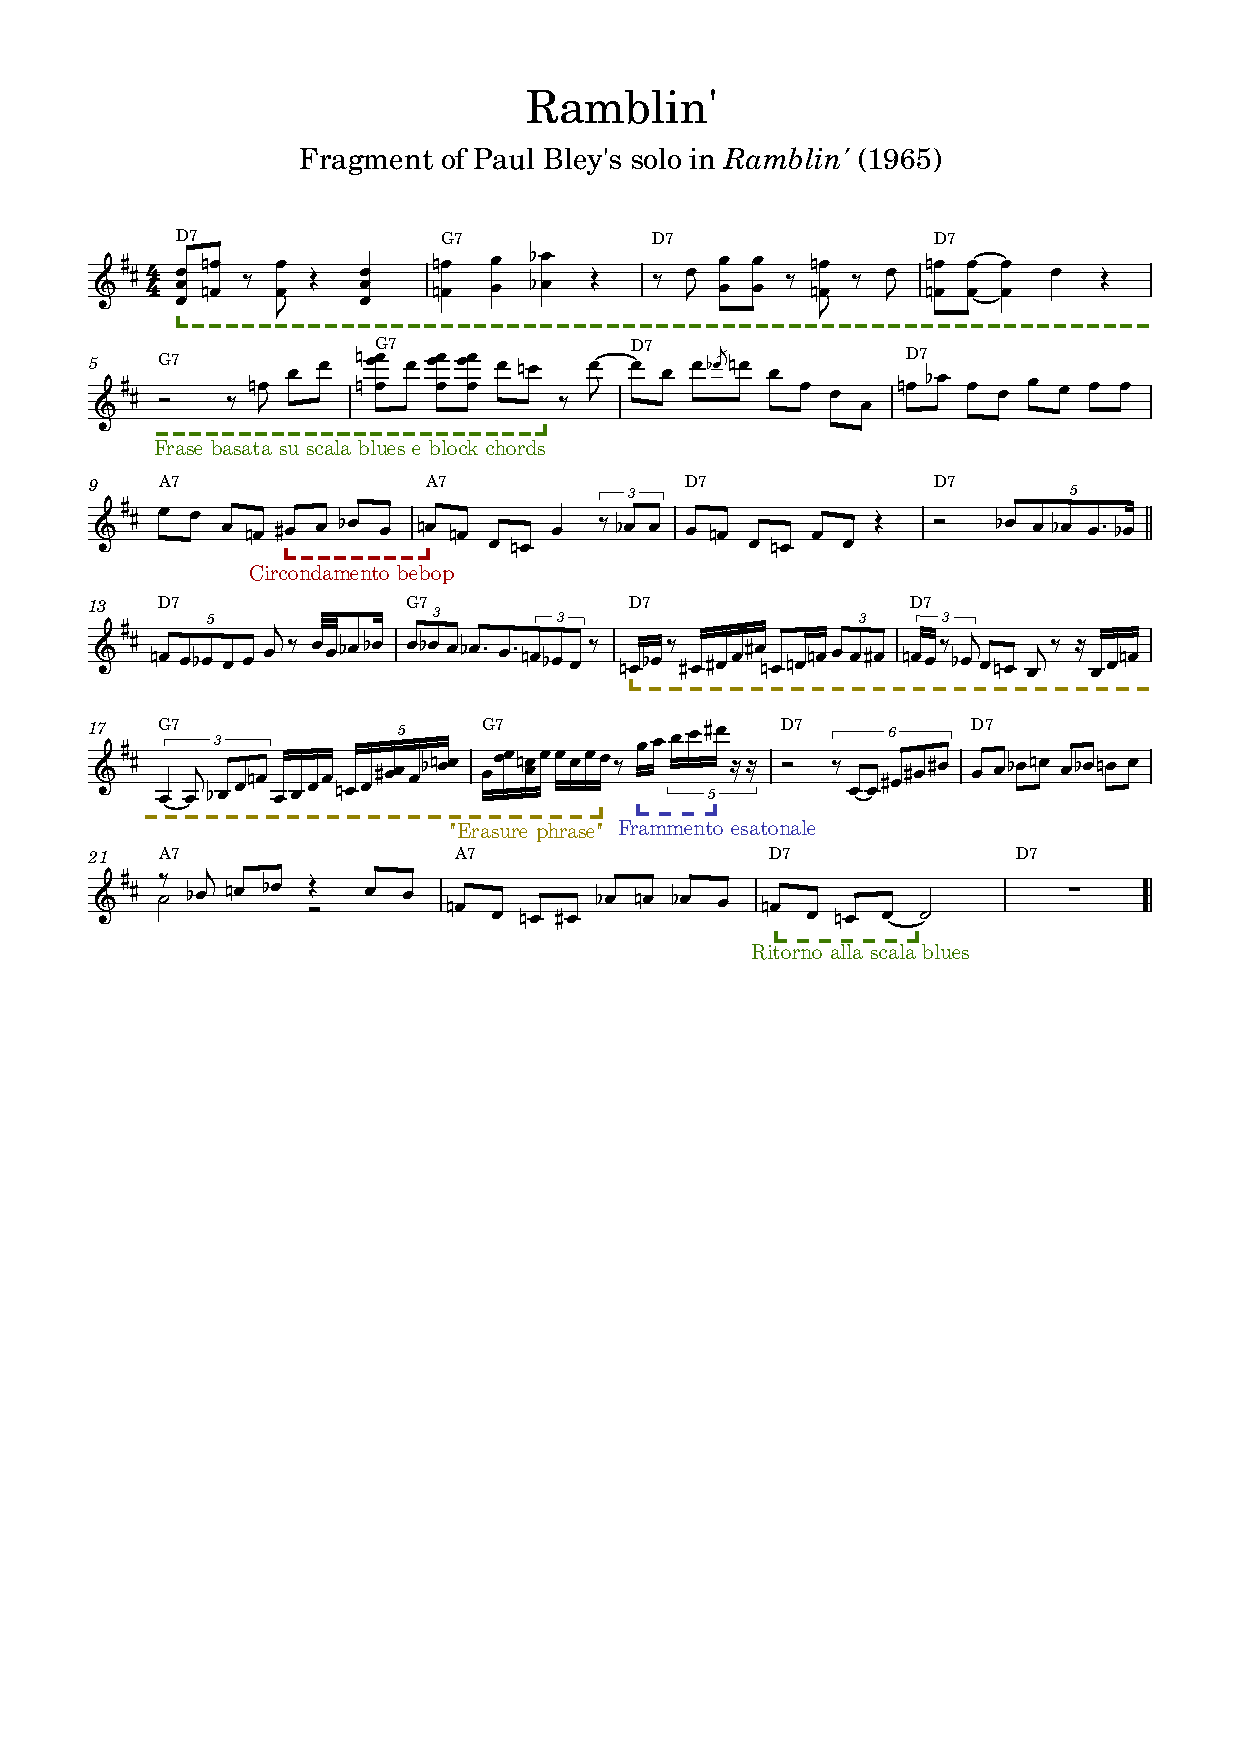
\includegraphics[clip,trim=1cm 13cm 1cm 3.5cm, width=\textwidth]{ramblin analysis.pdf}
	\caption{Ultimi due chorus di solo di pianoforte in \textit{Ramblin'}.}
	\label{fig:ramblin}
\end{figure}
Il blues è uno dei capisaldi dell'estetica di Coleman, per il quale costituiva sia un punto di partenza personale (come ex sassofonista di Rhythm \& Blues) sia culturale, nell'ambito di una musica che guarda a un ritorno alle radici dell'espressione afroamericana\footcite[38]{Cogswell1989}. Non stupisce quindi che anche Bley (seppur chiaramente per motivi diversi) torni così spesso e con tale limpidità al linguaggio blues. Dopotutto lui stesso riflette, a fronte della domanda di Arrigo Cappelletti sul suo rapporto con la tradizione blues:
\begin{fquote}
	Il blues è un ottimo punto di partenza per poter suonare tutte le forme di jazz. Quindi quando suoni frasi orientate al blues sei abbastanza certo che finirai sul tracciato del jazz.\footcite[135]{cappelletti}
\end{fquote}
\section{In caduta libera con Giuffre}
Oltre a Coleman, l'altra figura che Bley piazza nel suo pantheon di ispirazioni è Jimmy Giuffre\footcite{hamilton}. Il fatto che il pianista ponga queste due figure, ambedue pionieri e artefici di lavori all'apparenza così radicalmente diversi, è significativo dei punti in comune tra i due artisti.\par
Giuffre non era nuovo alle formazioni senza batteria (spesso note discograficamente come Jimmy Giuffre 3), come quella con il chitarrista Jim Hall alla cui dipartita si deve l'ingresso di Bley e Swallow nel trio. Giuffre conobbe Coleman (così come Bley) alla School of Jazz di Lenox nel 1959, fu l'unico musicista della scuola a farsi affascinare dalle suggestioni free del sassofonista tanto da decidere di modificare la traiettoria della propria musica (in maniera specifica, quella clarnittistica)\footcite[69]{litweiler}. A tal proposito ebbe da dire:
\begin{fquote}
	Avevo sentito molto parlare di lui, ma poi l'ho sentito suonare. Faceva le stesse cose che io stavo cercando, nel suo modo personale. La cosa meravigliosa a riguardo di questo aspetto è che non ha niente a che vedere con le idee o con il contenuto musicale, ma bensì con un'affermazione - e quando qualcuno arriva al punto di essere così libero e sicuro della propria affermazione, allora si tratta solo di parlare. Non è una competizione con nessun altro.\footcite{stephens}
\end{fquote}
Così come Bley stesso, l'incontro con il sassofonista texano aveva innescato una scintilla che avrebbe negli anni a seguire innescato un interesse nel free e in generale nell'improvvisazione libera. Infatti ancora più di Coleman, che in quegli anni si muoveva ancora stabilmente all'interno di orizzonti ritmici e armonici estesi seppur molto legati alle forme originarie del linguaggio jazz, il trio di Giuffre con Bley e Steve Swallow si prepone come la naturale evoluzione alla proposta di improvvisazione libera che Lennie Tristano, già nel 1949, aveva avanzato. Prendendo spunto dall'interesse del clarinettista per la musica cameristica, Bley ricorda come nel trio di Giuffre vigesse l'approccio che gli strumenti nel trio fossero voci eguali, dove ognuno aveva esattamente un terzo della responsabilità anzichè essere relegati ai ruoli convenzionali dell'accompagnamento jazz\footcite[389]{johnston}. Nelle note di copertina di \textit{Free Fall} Steve Swallow ricorda:
\begin{fquote}
	Passavamo tanto tempo parlando quanto suonando durante le nostre prove, ponendoci domande come: come possiamo suonare a una velocità data ma senza un tempo fisso? Quanto a lungo è possibile improvvisare senza far riferimento a una funzione tonica? Qual è la melodia più lunga che possiamo suonare senza interruzione?
\end{fquote}
La musica del trio si configura così come un importante collegamento tra le strutture più legate alla forma canzone e alla pulsazione jazzistica di Coleman e Ayler e agli improvvisatori di matrice europea, emersi più tardi verso la fine degli anni '60, quali Derek Bailey, Peter Brötzmann ed Evan Parker.\par
 Il trio aveva sviluppato un approccio all'improvvisazione sorprendentemente sistematico e preciso\footcite[387]{johnston}. A tal proposito Bley descrive le tecniche di prova come basate su ``premesse per l'improvvisazione'' nel senso di trattare aspetti e gesti musicali, interazioni e forme come materiali da manipolare anzichè come confini, come le forme compositive o il sistema temperato occidentale, entro cui limitare la propria tavolozza di suoni e decisioni\footcite[389]{johnston}. Giuffre aveva esplicitamente istruito Swallow a forzarsi non cadere all'interno di cadenze e risoluzioni classiche (come quella dal quinto grado alla tonica), consentendo quindi al basso di assumere una maggiore interattività melodica all'interno della formazione\footcite[390]{johnston}. Chiaramente, tali indicazioni riguardavano anche Bley, che senza alcun dubbio trasse da questa esperienza un grande influsso per quanto concerne la sua visione degli accordi come melodie verticali: ``[...] potevo suonare meno accordi e trattare il piano più come un fiato\footcite[390]{johnston}''. Un simile approccio era riservato al trattamento del tempo musicale, con Giuffre impegnato a condurre una decostruzione della pulsazione regolare che caratterizza la maggior parte del jazz senza però rigettarla: la sfida stava nel sviluppare la capacità di passare da uno scenario guidato da una pulsazione a uno più libero e ``avere la flessibilità di fare ciò che si voleva quando si voleva\footcite[390]{johnston}''. Swallow a tal proposito ricorda come il trio si interrogasse sulle diverse gradazioni nell'interpretazione del tempo o se fosse possibile che ognuno suonasse al proprio tempo indipendentemente da quello degli altri\footcite[390]{johnston}. A differenza dell'approccio più classico al free jazz, inoltre, Giuffre si prepose di porre una particolare attenzione alla tessitura timbrica dei tre strumenti e alle loro interazioni: ad esempio, Swallow ricorda un esercizio in cui il trio doveva suonare per dieci o quindici minuti attorno al do centrale, sovrapponendosi sullo stesso registro, per poi virare sull'orizzonte opposto in modo tale che il piano suonasse quanto più alto possibile rispetto al clarinetto e il basso raggiungesse invece il registro più grave in assoluto. In seguito, i musicisti avrebbero dovuto tratte le proprie conclusioni riguardo i territori timbrici e contrappuntistici in cui le diverse tecniche li avrebbero portati\footcite[391]{johnston}. \par
 Nonostante questo approccio molto orientato alla ricerca, anche intellettuale, e allo sviluppo di un vocabolario sonico da cui estrarre materiale a seconda delle esigenze, è bene notare come il linguaggio in realtà non si estranei mai in maniera radicale dalla tradizione jazz, costituendone un'estensione più che un rifiuto\footnote{Bley stesso sosteneva che il suo unico criterio decisionale per accettare o scartare materiale musicale fosse la sua ``validità in quanto jazz''.\cite[17]{heckman}}. Dopotutto, Swallow ricorda che ``non abbiamo mai inteso mancare di approvazione a \textit{Sonny Rollins at the Village Vanguard}; al contrario, avevamo reverenza per quelle cose\footcite[388]{johnston}''. Questo pone il progetto di Giuffre in contrapposizione con altri improvvisatori europei come Eddie Prevost e il già citato Bailey, che invece avevano deliberatamente deciso di prendere le distanze dal jazz. Per portare un esempio concreto, il brano \textit{Me Too} del disco \textit{Thesis} propone quello che di fatto è un blues la cui caratterizzazione viene solo accennata, rimanendo implicita (a differenza del ``country blues'' di \textit{Ramblin'} di Coleman). \par
 A tal proposito, è sempre interessante notare come nei primi due dischi (in particolare il primo, \textit{Fusion}) del trio di Giuffre vi sia la presenza di composizioni firmate da Carla Bley oltre la maggioranza di quelle composte da Giuffre: esse, come appare analizzando ad esempio \textit{Jesus Maria} e \textit{Ictus}, sono un sunto della visione compositiva di Carla Bley basata su temi modesti, trasparenti e armonicamente ambigui\footcite[25]{carla} che permettevano un'agevole esplorazione dei concetti di libertà armonica e ritmica.
 Si guardi, ad esempio, un passaggio dalla trascrizione del solo di pianoforte (che improvvisa, ovviamente, insieme al clarinetto) di \textit{Jesus Maria}, il brano firmato da Carla Bley che apre \textit{Fusion} (in figura \ref{fig:gesummaria}). Qui Bley alterna alla mano destra un fraseggio molto diradato e lirico con alcune occasionali frasi più veloci con funzione di \textit{erasure phrases}, non a caso proprio in corrispondenza della chiusura della sezione B di questo pezzo. Nonostante il brano, a differenza di quelli dal più radicale \textit{Free Fall} abbia in questo caso una pulsazione ritmica regolare scandita dal basso e dalla mano sinistra, si possono allo stesso modo apprezzare le dilatazioni e i restringimenti di tempo nella \textit{erasure phrase} così come la tendenza, che Bley avrebbe mostrato sempre da questo punto della carriera in avanti, ad alternare frasi lunghe con frammenti più episodici inframmezzati da pause, prassi inquadrabile nel tentativo di evitare di ricadere in cliché esplicitamente jazzistici\footcite[107]{dean}.
 \begin{figure}[h]
 	\centering
 	\includegraphics[clip,trim=1cm 13cm 1cm 2cm, width=\textwidth,page=2]{jesus solo-Piano}
 	\caption{Frammento dal solo di pianoforte di \textit{Jesus Maria}.}
 	\label{fig:gesummaria}
 \end{figure} 
 Dall'esperimento di Giuffre, senza alcun dubbio unico nel panorama jazzistico dell'epoca e a cui, forse, non venne tributato il giusto merito, emerge una musica allo stesso tempo intellettuale e spontanea. La melodia, fulcro del contrappunto, si frammenta nella dinamica del trio a tal punto da creare brevi macchie impressionistiche in continuo mutamento e, soprattutto, un continuo senso di tensione. In questo senso, con le continue ambiguità e escursioni armoniche rispetto al tema, la musica del trio ricade perfettamente nella summenzionata definizione di atonalità secondo Reti. Non stupisce l'importanza attribuita da Giuffre al concetto di affermazione, che la parola inglese \textit{statement} carica di un senso di oggettività ancora maggiore della traduzione italiana, dal momento che la natura placida e apparentemente innocua della musica appare come una pacata affermazione, in contrasto con il piglio battagliero e decisamente più rumorista del free jazz mainstream\footnote{Bley sostiene in \cite{hamilton} di essere in realtà un "urlatore free jazz" di indole più affine a Coleman che a Giuffre, offrendosi addirittura di urlare durante l'intervista; Hamilton, saggiamente, declina. Considerando, in ogni caso, anche la carriera successiva di Bley viene difficile dare credito a questa sua affermazione (così come a molte altre, a dire il vero).}. Giuffre, d'altro canto, viene dal cool jazz e così la sua improvvisazione libera è, anch'essa, cool: questa caratterizzazione, però, non deve trarre in inganno il lettore riguardo alla carica assolutamente innovativa di questa musica, sia sul campo ritmico che su quello armonico che su quello improvvisativo.
 
 \section{Più vicino: gli standard, i trii, i soli}
 Si può suggerire che l'incontro con Giuffre abbia costituito per Bley la chiave di volta per la formazione della propria musicalità e del proprio stile: se, infatti, Bley era un pianista completamente diverso prima del contatto di Coleman altrettanto si può dire dell'esperienza con il clarinettista. Ne è una dimostrazione il fatto che uno dei soli più celebri del pianista sia quello sullo standard \textit{All the Things You Are}, nel disco \textit{Sonny Meets Hawk!}. Nonostante lo scenario, se confrontato con quelli in cui Bley si era mosso fino a quel punto e in cui si sarebbe mosso in futuro, possa apparire particolarmente limitante date le velleità del pianista, è significativo come invece il solo sia la perfetta trasposizione su uno standard delle idee ritmiche e armoniche sviluppate fino a quel punto. Anche questo non deve sorprendere in luce della esplicita intenzione di Bley di aderire alla tradizione jazzistica piuttosto che rifiutarla: ciò include anche suonare gli standard. Il pianista ha nel suo catalogo più di uno sforzo dedicato al corpus di canzoni di cui la tradizione jazz si è appropriata: \textit{\textbf{My Standard}} [SteepleChase Records 1985], \textit{\textbf{Diane}} [SteepleChase Records 1985] con Chet Baker e \textit{\textbf{Out Of Nowhere}} [SteepleChase 1997] con Lee Konitz. Come nota Cappelletti\footcite[63]{cappelletti}, Bley è sempre stato affascinato dalle melodie e in particolare da quelle spezzate e immerse nel silenzio: tale approccio minimalista, unito alle già citate escursioni armoniche e ritmiche, caratterizza anche il suo approccio agli standard qualora il contesto, come nel caso del disco con Chet Baker, non richieda invece un approccio più tradizionale.\par
 Nel solo di \textit{All the things you are}, però, Bley non appare in alcun modo inibito dai suoi colleghi musicisti, che pure ha prima accompagnato durante i rispettivi soli con un approccio tutto sommato attinente alla tradizione. Il solo si apre con un'imitazione dell'ultima frase suonata da Hawkins, da cui poi Bley prende spunto per altre variazioni ritmiche basate sulla manipolazione della pulsazione (e infatti difficili da trascrivere con la notazione tradizionale\footnote{Bley ricorda come il fatto che i soli di Coleman non fossero trascrivibili in maniera agevole aveva attratto delle critiche, ma ``la colpa era dei limiti tecnici della notazione musicale, non di Ornette''. \cite[67]{stopping}.}).
 \begin{figure}[H]
 	\centering
 	\includegraphics[clip,trim=1cm 21cm 1cm 3.3cm, width=\textwidth,page=1]{things u are anaylisi}
 	\caption{Inizio del solo di pianoforte di \textit{All the Things You Are}.}
 	\label{fig:screenshot002}
 \end{figure}
 Come è possibile apprezzare in figura \ref{fig:screenshot002}, in battuta 7 Bley sovrappone a un accordo di \verb*|Cmaj7| un arpeggio di \verb*|Emaj7|. In generale, più della metà delle battute del solo presenta materiale che non corrisponde all'accordo della struttura e che a volte pare esistere su un piano armonicamente parallelo.\par
 Bley, inoltre, fa largo uso di progressioni, toni ripetuti e intervalli ampi\footcite[108]{dean}.
 \begin{figure}[h]
 	\centering
 	\includegraphics[clip,trim=1cm 2cm 1cm 19.2cm, width=\textwidth,page=1]{things u are anaylisi}
 	\caption{Frammento del solo di \textit{All the things you are}.}
 	\label{fig:screenshot003}
 \end{figure}
 Nel caso mostrato in figura \ref{fig:screenshot003}, la progressione è basata su un moto cromatico della nota inferiore della melodia che, insieme ai toni ripetuti dalla mano sinistra, va a formare armonie di tritoni e quarte (in fin dei conti non troppo dissimili da quelle presenti nell'introduzione di \textit{I can't get started} in figura \ref{fig:cant}). Simili espedienti possono essere ravvisati verso la fine del solo (come nell'esempio di figura \ref{fig:screenshot004}) dove si assiste anche a un maggiore utilizzo di rapide frasi con il valore di \textit{erasure phrases}.\par
 Si assiste così a un sovvertimento radicale del concetto di armonia e ritmo all'interno dello standard, tonale per eccellenza, ma a un esame più attento non sfugge come in realtà Bley accolga nel suo solo anche diverse tecniche tradizionali come le citazioni dai soli del contesto della performance, il recupero di materiale tematico dalla melodia, il fraseggio continuo e, a conti fatti, della tonalità e delle scale tipiche del dizionario boppistico.
 \begin{figure}[H]
 	\centering
 	\includegraphics[clip,trim=1cm 10.3cm 1cm 10cm, width=\textwidth,page=3]{things u are anaylisi}
 	\caption{Frammento del solo di \textit{All the things you are.}}
 	\label{fig:screenshot004}
 \end{figure}
Sempre in questo periodo, che corrisponde inoltre alla separazione con Carla Bley che costituì per il pianista un avvenimento particolarmente sofferto\footcite[68]{cappelletti}, Paul Bley inizia con \textit{Closer} una serie di registrazioni in trio. È stato già detto come questa formazione fosse risultata particolarmente affine alla ricerca della libertà improvvisativa tanto cara a Bley: ancora di più che con Jimmy Giuffre, il trio classico lascia completamente le redini dell'improvvisazione (e in generale, del brano) in mano al pianista; allo stesso tempo questo tipo di formazione permette atmosfere sommesse e aperte che Bley, su cui la lezione di Giuffre doveva senz'altro aver trovato terreno fertile, ha sempre mostrato di prediligere. \\
I parallelismi con i lavori registrati insieme al clarinettista non mancano: sebbene la divisione dei ruoli appaia più tradizionale, è innegabile notare che la gerarchia di ruoli che mantiene il pianoforte saldamente al comando sia spesso flessibile: in \textit{Closer} il basso di Steve Swallow e la batteria di Barry Altschul spesso assurgono al ruolo di co-improvvisatori (come ad esempio nel brano \textit{Batterie}) interagendo nella libertà tonale e ritmica che già aveva caratterizzato i dischi con Giuffre.\\
Come già accennato in precedenza, la metodologia impiegata da Bley per \textit{Closer} consisteva nello spingere i musicisti a eseguire soli estremamente corti prima di ritornare all'esposizione tematica: ne risultarono brani molto corti, con strutture aperte e in bilico, quasi con la qualità della bozza. Si tratta di dischi che si potrebbe definire minimalisti in un senso diverso da quello comunemente inteso di minimalismo americano (la corrente compositiva che include autori quali Steve Reich e Philip Glass), in quanto si ha l'impressione che i brani e le improvvisazioni progrediscano per piccole aggiunte e variazioni attorno nuclei armonici e melodici\footcite[33]{cappelletti}. Si sviluppa, anche in questo caso, il tipico stile pianistico bleyiano che accosta continuità e fratture: le linee melodiche possono avere una durata di più battute, estendendosi anche oltre la scansione ritmica della batteria, per poi essere improvvisamente interrotte; le melodie possono avere una natura estremamente cantabile per poi proseguire con passaggi fuori tonalità o intervalli ampi e inaspettati.
 \begin{figure}[h]
	\centering
	\includegraphics[clip,trim=1cm 10cm 1cm 7.5cm, width=\textwidth,page=1]{ida_analisi}
	\caption{Frammento del solo di \textit{Ida Lupino}}
	\label{aida}
\end{figure}
Il frammento di improvvisazione in figura \ref{aida} mostra un esempio dell'applicazione di queste tecniche e, in generale, di un lirismo estremamente presente ma allo stesso tempo ambiguo e libero dai vincoli di tempo e di tonalità. Spesso Bley durante i soli cambia improvvisamente registro sulla tastiera (come si può ascoltare nel brano \textit{Start}) e in generale si mostra capace di invertire repentinamente la rotta dell'improvvisazione imponendo un'alternanza di atmosfere sfruttandone il contrasto. Parte del fascino del pianismo di Bley sta proprio nel trovare una continuità anche nella rottura e nella discontinuità, superando l'apparente dicotomia tra il fraseggio jazzisticamente melodico e la frammentarietà del free.\par
In \textit{Closer} quasi tutte le composizioni sono firmate da Carla Bley; fanno eccezione \textit{Crossroads} (di Ornette Coleman) e \textit{Cartoon} (di Annette Peacock). Paul Bley, per tutta la vita, avrebbe continuato a suonare i brani composti dalle sue due (ex) mogli, con una particolare predilezione per le composizioni di Carla Bley. Questo non è un caso: a fronte di una generale aridità di Paul come compositore nel senso classico del termine. È già stato accennato come egli fosse più interessato all'idea di composizione estemporanea nella forma di improvvisazione (è quasi impossibile trovare partiture di temi scritte su carta\footcite[24]{cappelletti}) e le composizioni di Carla offrono invece un ottimo terreno per l'improvvisazione di Bley: brani concisi, di Weberniana memoria\footcite[22]{carla}, con armonie composte dal raggruppamento di elementi semplici (molto spesso triadiche), melodie estremamente cantabili che però spesso escono dagli schemi accordali, riferimenti a tradizioni folk come quella spagnola e sudamericana, passaggi dotati di una velata e cinica ironia; si tratta di composizioni spesso minime, con inaspettate pause e inversioni sempre in bilico tra quelli che Beal ha definito i due lati di Carla Bley: quello dionisiaco (ravvisabile in composizioni come \textit{Ictus}) e quello apollineo (che traspare da brani come \textit{Ida Lupino}) \footcite[18]{carla}. Non stupisce, in tal senso, che Paul abbia sempre amato e suonato i brani di Carla Bley. \par
\begin{figure}[h]
	\centering
	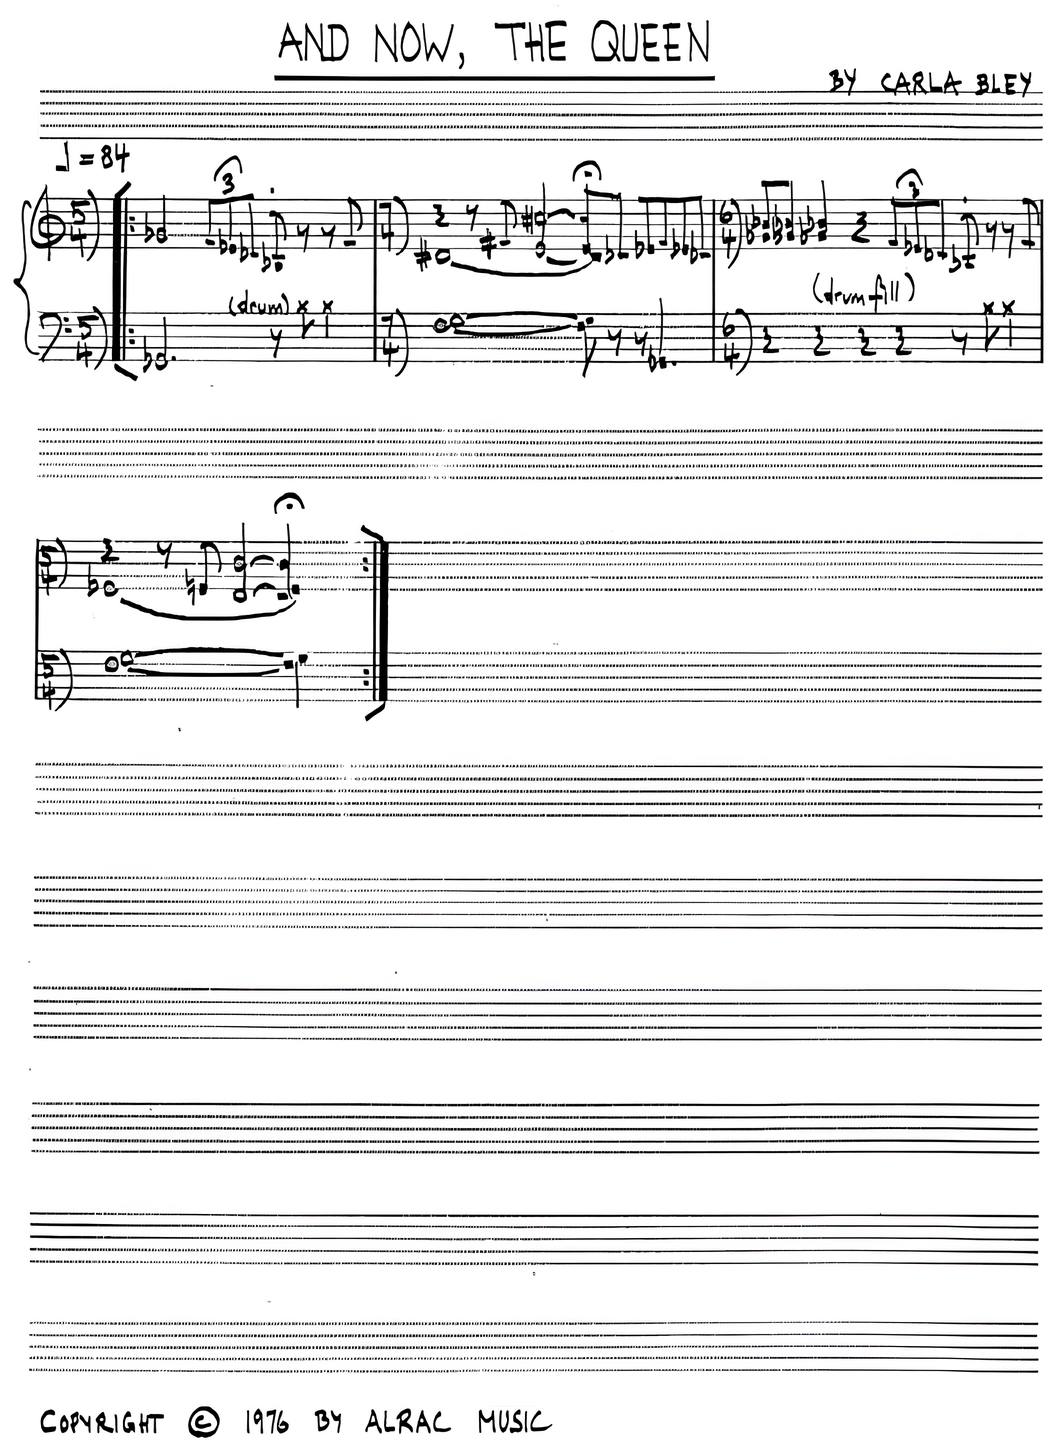
\includegraphics[width=\textwidth, clip,trim={0cm 25cm 0cm 0cm}]{screenshot005up}
	\caption{Tema di \textit{And now, the Queen} di Carla Bley.}
	\label{nowthequeen}
\end{figure}
Un brano che esemplifica egregiamente le caratteristiche dello stile compositivo di Carla Bley è \textit{And now, the Queen} (figura \ref{nowthequeen}\footcite{earlycomp}), eseguito da Paul Bley sia in trio (nel disco \textit{Closer}) che in solo (nel disco \textit{Alone, again}). In sole quattro battute Carla Bley realizza un capolavoro\footnote{Swallow riteneva che questo brano fosse tra i più rilevanti di Carla Bley. \cite[23]{carla}.} di minimalismo e laconicità. Facendo seguire a passaggi fortemente tonali, dal piglio solenne e quasi marziale, sezioni in cui l'armonia si disgrega per diventare interrogativa. Le due anime del pezzo si scontrano in uno scenario che, se contestualizzato con il titolo, non manca di una certa velata ironia (altro tratto tipico della compositrice). Il pezzo non ha una vera e propria tonalità e l'indicazione metrica, che cambia a ogni battuta, ne acuisce l'ambiguità sul piano ritmico oltre che melodico. Nonostante tutte queste caratteristiche è però innegabile che il brano sia fortemente lirico dall'inizio alla fine: le inversioni di tonalità e di metro concorrano a questo scopo piuttosto che avere un più semplice ruolo di spaesamento.\\
Carla Bley è stata una compositrice a metà tra due mondi: quello europeo, a cui si sentiva legata per inclinazione, e quello del jazz americano, a cui era legata per il contesto culturale in cui si trovava\footnote{Bley, avendo sviluppato un crescente rancore verso quello che riteneva l'auto-compiacimento del free jazz, era arrivata a definirsi ``arrabbiata con il jazz''. \cite[34]{carla}.} e forse, proprio per questo, ingiustamente trascurata da entrambe le sfere.\par
La forma del trio non avrebbe mai abbandonato Paul Bley: se il disco \textit{Ramblin'} del 1966 mostra una formazione interessata a un approccio più tradizionale (con pezzi latin come \textit{Mazatlon} e blues come \textit{Ramblin'} di Coleman) ma sempre attenta alla tensione tra armonia e ritmo, con un continuo alternarsi di atmosfere e registri, nel disco \textit{\textbf{Memoirs}} [Soul Note 1990] (anch'esso registrato in Italia con Charlie Haden al basso e Paul Motian alla batteria) si ha un esempio di come un Bley più tardo interagisce con la forma del trio. In questo caso si vive un ambiente musicale più sobrio e riflessivo, con un approccio più trattenuto e all'apparenza tradizionale tipico della fase più recente della carriera del pianista, ma che non si nega le libertà ritmiche e armoniche che hanno sempre caratterizzato il suo modo di suonare. Sostenuti dalla batteria minimale e impressionistica di Motian, pezzi come \textit{Insanity} e \textit{Latin Genetics} (quest'ultimo, ancora, di Coleman) mostrano un Bley forse meno ansioso di rompere barriere, ma anche più a suo agio nel linguaggio per cui tanto ha faticato in gioventù. Un altro esempio interessante di trio si può trovare nel disco \textbf{\textit{BeBopBeBopBeBopBeBop}} [SteepleChase Records 1990] con Bob Chainsaw e Keith Copeland, un interessante omaggio ai classici del bebop in cui emerge il già citato legame di Bley con gli standard della tradizione jazz: già dalla prima traccia, una versione del blues \textit{Now's the Time} di Parker emerge un Bley completamente a suo agio in brani tradizionali per eccellenza, senza per questo scendere a compromessi con il proprio stile distintivo.\par
Il primo album di pianoforte solista di Bley risale al 1972. Come molti avvenimenti nella sua carriera, nacque quasi per caso da una fortuita richiesta di Manfred Eicher della ECM. Bley sostiene:
\begin{fquote}
	Il pianoforte solo è diverso da suonare in un gruppo ed è anche diverso dal suonare in solo su altri strumenti. Ogni periodo storico è stata identificato da un modo di suonare il piano quasi completamente diverso dagli altri.[...] L'unica cosa che noi [Bley e Eicher] avevamo bisogno di sapere riguardo al futuro del pianoforte solista era: ciò che era stato fatto prima. Le decisioni su cosa fare sono ancora completamente aperte e non ci sono precedenti.\footcite[154]{stopping}
\end{fquote}
Pur personalmente intenzionato a volersi muovere attraverso tutti gli stili jazzistici\footcite[5]{smith}, anche nel piano solo Bley voleva porsi come un innovatore e a tale scopo sfruttò le tecniche di registrazione innovative di Eicher per massimizzare il sostegno delle note e degli armonici\footcite[154]{stopping}, memore delle proprie esperienze sia con gli strumenti elettronici che con il sax non temperato di Coleman. \par
Riguardo all'improvvisazione solistica Ed Sarath ritiene che l'improvvisazione solistica, in quanto non soggetta all'influenza di eventi esterni, sia un'attuazione della spinta improvvisativa meno soggetta alle dinamiche di ciò che egli chiama consapevolezza ritensiva-protensiva\footcite[6]{edsarath}, vale a dire il processo creativo che porta a proiettare l'improvvisatore su coordinate temporali\footcite[27]{edsarath}, che di fatto avvicina l'improvvisazione a una forma di composizione estemporanea. A tal proposito si fa notare come le composizioni soliste di Keith Jarrett siano a volte indistinguibili, sul piano della coerenza temporale e strutturale, dalle sue improvvisazioni solistiche mentre lo stesso non si può dire delle improvvisazioni e delle composizioni per trio, che chiaramente differiscono per la tendenza ad aderire a un referente\footcite[20]{edsarath}.\par
Per quanto concerne Paul Bley, questo pensiero è applicabile al fatto che nel suo piano solo si assiste ad alcune delle caratteristiche del suo pianismo nelle forme meno adulterate\footcite[80]{cappelletti}. Il disco \textit{Open, to Love} è pervaso di un profondo lirismo che non emerge con altrettanta frequenza nelle altre formazioni. Secondo Cappelletti, nei dischi solisti di Bley tutto è costruito nel momento stesso in cui appare all'ascoltatore, come se il pianista imparasse nuovamente a suonare il pianoforte ogni volta che vi si siede davanti\footcite[82]{cappelletti}. Vi è anche un particolare gusto, non scevro di intenzioni ironiche, per il citazionismo e la riproposizione di materiale tipico del vocabolario jazzistico, di intervalli, frasi e temi che diventano ambigui e fuori contesto\footcite[83]{cappelletti}. \textit{Open, to Love} contiene tre brani di Carla Bley, due di Annette Peacock e due originali (\textit{Started} e \textit{Harlem}). Nella forma del piano solo Bley adotta diverse strategie riguardo alle composizioni che interpreta: \textit{Closer} presenta un'improvvisazione fedele al tema; \textit{Ida Lupino} invece si avventura in territori blues e armonicamente divergenti dal pedale armonico, tra cui si scorgono frammenti di tema riproposto tra progressioni più convenzionali (con una piccola citazione a \textit{All the Things You Are}). Il brano in chiusura \textit{Nothing Ever Was, Anyway} a firma di Peacock è il perfetto sunto del pianismo solista di Bley: lunghi silenzi, sparute note che tracciano i contorni di armonie solo apparentemente elementari.
\section{Doppia unità: l'esperienza elettronica}
Annette Peacock, riguardo all'uso del sintetizzatore Moog:
\begin{fquote}
	È vero, abbiamo un nuovo suono, che proviamo ad ottenerlo o meno. È qualcosa di intrinseco allo strumento in sè, quindi non è più una preoccupazione. Ciò che cerchiamo di fare è dargli una forma e fare musica, dato che il medium non basta se non si ha una concezione e un approccio ben preciso alla musica.\footcite[16]{fiofori}
\end{fquote}
Bley scoprì, durante un'intervista per il magazine \textit{Downbeat} nel 1969, dell'esistenza dei sintetizzatori a tastiera\footcite[108]{stopping}. La notizia gli suscitò curiosità: fino ad allora la visione di costruttori quali Robert Moog e Donald Buchla, rispettivamente padri di quelle che oggi vengono chiamate ``east-coast synthesis'' e ``west-coast synthesis'' era stata per lo più orientata al mondo della composizione elettroacustica in ambito accademico, nel solco tracciato da compositori come Karlheinz Stockhausen e Pierre Schaeffer\footcite[305]{gluck}. Mentre Buchla avrebbe continuato a progettare sintetizzatori con interfacce utente particolari e non orientati necessariamente all'utilizzo da parte dei tastieristi, in quegli anni Moog stava sperimentando con l'introduzione di controlli a tastiera per facilitare l'adozione dello strumento anche in ambito di registrazione in studio e di performance di popolar music\footcite[15]{fiofori}. Chiaramente, all'epoca i sintetizzatori modulari erano pesanti, difficili da trasportare, impossibili da mantenere accordati e privi della possibilità di salvare le configurazioni (le cosiddette \textit{patch} ottenute collegando gli output dei segnali CV, control voltage, dei diversi moduli agli input di altri moduli) e tanto meno richiamarle da una memoria. \par
Non è chiaro esattamente come Bley abbia ottenuto il sintetizzatore da Moog. Nella sua autobiografia egli sostiene di aver convinto il produttore a elargirgli un sintetizzatore sostenendo che l'azienda non avrebbe avuto il futuro se lo strumento non fosse stato visto come utilizzabile da un musicista \textit{on the road}\footcite[110]{stopping}. Ci si può interrogare su quale completo tracollo a livello di marketing sia stato dipinto a Moog per convincerlo a cedere con tanta generosità uno strumento dal costo esorbitante allo semisconosciuto Paul Bley, pianista di avanguardia e apparentemente unica persona negli Stati Uniti a suonare uno strumento a tastiera professionalmente. Senza nulla togliere alla liberalità dell'uno nè alle doti persuasive dell'altro, si può dire che ci sono motivi di dubitare della versione proposta da Bley\footnote{\cite[307]{gluck}. In generale, Bley soffre (insieme a molti colleghi della sua generazione) di quel gusto per l'aneddoto dal sapore leggendario che a volte lo spinge a dichiarazioni poco appropriate.}. In ogni caso, Bley ottenne un sintetizzatore e a suo dire impiegò, insieme a Peacock, i primi due anni di possesso per capire l'interfaccia e i principi di sintesi\footnote{\cite[109]{stopping}. Anche qui, Bley con ogni probabilità sta esagerando. Due anni sono un tempo decisamente eccessivo per capire il funzionamento di un sintetizzatore sottrattivo. Anche a fronte di eventuali difficoltà tecniche che avessero potuto presentarsi, Bley era lungi da essere uno degli \textit{early adopters} dello strumento. Dal momento che non viveva in stato di segregazione dal resto della società americana, non è chiaro perchè non avrebbe dovuto chiedere aiuto a figure come Herb Deutsch che da tempo impiegava il sintetizzatore Moog nelle performance live (\cite[307]{gluck}). È probabile che Bley abbia preferito dipingersi come vincitore di un'epica lotta tra uomo e tecnologia piuttosto che raccontare fedelmente i fatti.}. \par
Il rapporto tra Bley e il sintetizzatore è breve ma intenso. Tra il 1969 e il 1972 Bley registra dieci album basati sull'utilizzo dell'elettronica, con risultati sorprendentemente vari a livello di soluzioni tra free jazz (come l'album \textit{Improvisie}), fusion (come l'album \textit{\textbf{Paul Bley \& Scorpio}} [Milestone 1973], che sembra anticipare in alcuni punti il lavoro di Jan Hammer con Billy Cobham) e anche pop (\textit{\textbf{The Paul Bley Synthesizer Show}} [Milestone 1971]).\par
Il sintetizzatore permise a Bley di avere controllo su un range di tecniche di performance rispetto al pianoforte. Finalmente, anch'egli poteva come Coleman iniziare ad abbandonare la rigida griglia del sistema temperato occidentale con quella stessa mentalità che lo spingeva ad esplorare i suoni interni del pianoforte tramite le tecniche estese. Altro punto focale dell'approccio di Bley al sintetizzatore è l'attenzione al sostegno dei suoni (lo stesso che aveva chiesto a Eicher in fase di registrazione di \textit{Open, to Love} che non casualmente risale allo stesso periodo) e alla capacità di programmarne l'evoluzione nel tempo attraverso le tecniche del bending, del \textit{syncing} della frequenza tra due oscillatori, del portamento, della distorsione e della modulazione tramite LFO, \textit{ring modulators} e generatori di inviluppo\footcite[317]{gluck}. Chiunque abbia avuto l'opportunità di approcciarsi al sintetizzatore da pianista riconoscerà in questi aspetti il superamento dei classici limiti dello strumento acustico. È interessante notare come anche sul sintetizzatore Bley spesso prediliga repentini cambi di registro e anche di suono, amplificando la tendenza all'esplorazione timbrica che già aveva iniziato sul pianoforte. Bley spesso fa uso, in maniera non sorprendente, di un timbro molto vocale, simile a quello di un fiato (come un sassofono soprano o un clarinetto) che ben si presta alla proiezione vocale della frase solista, cosa non altrettanto facile sul pianoforte\footcite[317]{gluck}. In particolare, si può ascoltare come nella performance di coppia di \textit{Touching}, contenuta nell'album \textit{Improvisie}, vi sia un esplicito contrasto tra il suono di Bley, più solistico, e quello di Peacock, che invece sceglie un timbro distorto a basse frequenze incrementando progressivamente la distorsione\footcite[318]{gluck}.\\
La scelta di coniugare diversi suoni attraverso l'utilizzo di strumenti multipli (quello che lui chiama ``keyboard sandwich'', di cui sostiene di essere l'inventore\footnote{\cite[113]{stopping}. Falso, con tutta probabilità.}) è un'altra caratteristica del suono elettronico di Bley: la melodia serpeggiante di \textit{Nothing Ever Was, Anyway} in \textit{The Paul Bley Synthesizer Show} è suonata alternando un sintetizzatore con un piano elettrico; la maggior parte del disco \textit{Paul Bley \& Scorpio}, di inclinazione più fusion, vede Bley alternarsi costantemente tra sintetizzatore, piano elettrico e pianoforte acustico. \par
Alcune caratteristiche del pianismo di Bley ben si traslano sulla tastiera del sintetizzatore: le \textit{erasure phrases}, confuse dal portamento, diventano vere e proprie macchie timbriche dall'effetto disorientante; le lunghe melodie inframmezzate da silenzi diventano paesaggi sonori meditativi in continua evoluzione; i contrappunti improvvisativi diventano non più solo melodici ma anche timbrici. In generale, l'approccio di Bley non è banalmente quello di un pianista a cui viene dato un sintetizzatore: si tratta, invece, di una vera esplorazione di uno strumento musicale distinto. È forse questo il merito principale del pionierismo di Bley (e di Peacock, ovviamente).\par
Bley avrebbe abbandonato poi quasi completamente l'elettronica. A motivarlo in questa scelta furono probabilmente le molte difficoltà comportate dal fare tour con uno strumento del genere, sempre pronto a imprevisti e malfunzionamenti\footcite[114]{stopping}. Bley ricorda come l'uso dei sintetizzatori gli valse l'esilio dallo storico locale Village Vanguard: 
\begin{fquote}
	Avevo il sintetizzatore sul palco, il trio che aspettava di suonare, il pubblico che aspettava che iniziassimo e io ero sul pavimento che guardavo sotto il sintetizzatore con una torcia tascabile e un cacciavite, chiedendo al pubblico attraverso il microfono della sala di avere cortesemente pazienza. Max Gordon mi disse tre cose: vai fuori, restaci e non tornare.
\end{fquote}
Ironicamente, poco dopo la rinuncia da parte di Bley agli strumenti elettronici furono messi in commercio sintetizzatori come il Minimoog e l'ARP Odyssey, esplicitamente pensati per essere portati in tour\footcite[321]{gluck}. \par Peacock avrebbe continuato nell'esplorazione elettronica con il disco \textit{I am the One}, i cui timbri pionieristici (uniti alla tecnica di modulazione attraverso un microfono) rendono chiaro quanto abbia pesato il ruolo della compositrice nel definire sonorità che ancora oggi si distinguono da quelle che la maggior parte dei lavori elettronici dell'epoca mostra. 
Riguardo a Bley non sarebbe mancato qualche sporadico ritorno all'elettronica come il disco \textit{Synth Thesis} del 1997 (realizzato con un sintetizzatore digitale: Bley ricorda lo stupore nel constatare la facilità d'uso rispetto alla sua esperienza con l'analogico\footcite[148]{stopping}). Un altro disco estremamente interessante è \textit{\textbf{The Paul Bley Quartet}} [ECM 1987] con John Surman (sassofono e clarinetto basso), Bill Frisell (chitarra) e Paul Motian (batteria). Si tratta di un'interessante unione tra l'improvvisazione libera cameristica alla Giuffre (con la conseguente dissoluzione dei ruoli dell'ensemble jazz classica: in questo caso manca completamente il basso) con le ambigue atmosfere elettroniche, questa volta date dalla chitarra modificata di Frisell.
\chapter{Breve analisi di tre brani: Ramblin', Jesus Maria e Ida Lupino}
In questa sezione verrà compiuta una breve analisi compositiva e stilistica dei tre pezzi presentati durante la prova finale di esecuzione pianistica. Si tratta di tre pezzi scelti nel periodo centrale, nel pieno dell'attività sperimentale, della carriera di Paul Bley. 
\section{Ramblin'}
\textit{Ramblin'} è un blues esteso composto da Ornette Coleman. Il tema originale, come suonato da Coleman, è il seguente:
 \begin{figure}[H]
	\centering
	\includegraphics[clip,trim=1cm 18cm 1cm 3.5cm, width=\textwidth,page=1]{ramblin coleman}
	\caption{Tema di \textit{Ramblin'} presente nel disco di Ornette Coleman \textit{Change of the Century} [Atlantic Records 1960].}
	\label{ramblcol}
\end{figure}
Questo pezzo, registrato con Bley all'Hillcrest Club ancor prima che con il quartetto classico di Coleman con Charlie Haden (basso), Billy Higgins (batteria) e Don Cherry (tromba e cornetta)\footcite[71]{litweiler}, è basato sulla forma blues arcaica. Là dove il jazz ha consacrato e cristallizzato la forma blues in 12 battute, Coleman opera un ritorno alle origini campestri e rurali di questa forma espressiva afroamericana, in cui la forma tripartita basata su un pattern tematico \verb*|AAB| (che in questo caso viene effettivamente conservato) non è determinata dalla struttura armonica, ma dal materiale melodico: riconnettendo il vero significato della parola \textit{blues} (vale a dire uno stato d'animo, in contrasto con la definizione ``intellettualizzata'' data a posteriori dai musicisti jazz), Coleman aderisce al principio di molti musicisti di blues rurale in cui il passaggio dalla tonica alla sottodominante e alla dominante è dipendente esclusivamente dalla lunghezza della frase cantata\footcite[38]{Cogswell1989}.\par
 \begin{figure}[h]
	\centering
	\includegraphics[clip,trim=1cm 11cm 1cm 3.3cm, width=\textwidth,page=1]{ramblin bley}
	\caption{Tema di \textit{Ramblin'} presente nell'album omonimo di Paul Bley}
	\label{ramblbley}
\end{figure}
Così la forma blues tripartita di \textit{Ramblin'} non viene suddivisa in tre gruppi da quattro battute ma bensì viene organizzata attorno alle tre frasi tematiche con lunghezza variabile (come dimostra l'ultima battuta in un metro accorciato rispetto al $\frac{4}{4}$ del brano). Le pause tra i frammenti tematici sono inframezzate dallo \textit{strumming} di Charlie Haden, in un chiaro riferimento alla musica folk americana e all'uso di strumenti a corda quali il banjo e la chitarra. Anche durante il solo di Coleman Haden accompagna alternando dodici battute di pattern di \textit{strumming} e sedici di più tradizionale \textit{walking bass} mentre Coleman raggiunge le tensioni della sotto-dominante e della dominante in maniera apparentemente slegata dal processo di accompagnamento del basso. In maniera simile, il solo di basso (accompagnato da un suono di campanello) consiste in un pedale di re su cui Haden suona liberamente, sempre in \textit{strumming}, delineando melodie estremamente semplici dal punto di vista ritmico e melodico. Tale approccio è, in maniera affascinante, molto vicino a quello che negli anni '70 sarebbe stato adottato dai musicisti vicini alla corrente del primitivismo americano (seppur con diverse premesse) quali Robbie Basho e John Fahey.\par
Questo ammaliante blues delle praterie visto dagli occhi di un quartetto jazz è realizzato da Paul Bley in maniera lievemente differente, come si può notare in figura \ref{ramblbley}.
In questo caso, l'accompagnamento al basso di Mark Levinson e alla batteria di Barry Altschul si configura come più tradizionale, pur rimanendo fisso su un pedale di re come nel brano di Coleman. Bley, oltre ad applicare qualche modifica alle note del tema, allunga gli spazi tra i frammenti tematici, utilizzandoli per \textit{fill} fortemente ritmici di lunghezza libera. Come si nota nel solo, trascritto in appendice \ref{solo:ramblin}, per Bley questo pezzo è l'occasione di fare uno sfoggio relativamente indisturbato del suo ricco vocabolario blues, qui realizzato in struttura fissa (a differenza della versione di Coleman). Le frasi utilizzano molti riff rinforzati da block chords a ottava (con quinta o sesta interna) ed è interessante notare, dopo una parte centrale più sommessa limitata a un registro più grave, la progressione del solo in direzione di una sempre maggiore apertura armonica (ma non ritmica) per poi chiudere con una lunga \textit{erasure phrase} al culmine della tensione, Segue il solo di basso di Levinson, su pedale di re, per poi chiudere con l'esposizione del tema.
\section{Jesus Maria} 
Il pezzo è uno dei primi lavori di Carla Bley, appartenenti a una fase in cui la compositrice lavorava in maniera quasi ossessiva alle sue composizioni, sviluppando un rapporto quasi simbiotico con il pianoforte (tanto che Paul Bley doveva lottare per prenderne possesso)\footcite[89]{stopping}. Costituisce uno dei primi lavori della compositrice a raggiungere una notevole popolarità\footcite[26]{carla}. A tal proposito Bley stessa disse:
\begin{fquote}
	Credo avessero un'anima leggermente diversa, data dalla mia formazione non ortodossa. Ero riuscita a mantenere la mia ignoranza, qualcosa che non puoi più riavere indietro una volta persa.\footcite[14]{carla}
\end{fquote}
Il brano fu registrato da Giuffre quasi immediatamente dopo che Bley lo ebbe scritto\footcite[26]{carla}; fu in seguito registrato, con una ricca sezione orchestrale che includeva una sezione di ricetrasmittenti, per l'album \textit{\textbf{Musique Mecanique}} [ECM 1979] e ancora più tardi, in versione per basso, pianoforte e quintetto di ottoni, per l'album \textit{\textbf{Carla's Christmas Carols}} [ECM 2009]. Il pezzo ha un sapore di musica folk spagnola (riecheggia \textit{Flamenco Sketches} di Miles Davis) testimone dell'interesse per Bley per la musica tradizionale (in particolare per quella iberica).\par
\begin{figure}[H]
	\centering
	\includegraphics[clip,trim=1cm 2cm 1cm 3.3cm, width=\textwidth,page=1]{Jesus maria theme}
	\caption{Tema di \textit{Jesus Maria} presente nell'album \textit{Fusion} di Jimmy Giuffre.}
	\label{jesusmariatheme}
\end{figure}
Un aneddoto interessante su questo brano è il fatto che esso costituisca la prima delle numerose commistioni, tipiche di Bley, tra le proprie composizioni, la poesia e la voce in generale: \textit{Jesus Maria} fu infatti inclusa in un libro di canzoni natalizie per cui Bley era stata assunta per scrivere gli arrangiamenti di pianoforti e la compositrice dovette quindi corredarla di un testo. Tecnicamente, questo rese anche \textit{Jesus Maria} la prima composizione di Bley pubblicata ufficialmente\footcite[33]{carla}.\par
La forma originale è una canzone ABABA\footcite[26]{carla}, ma nel disco di Giuffre viene suonata come $\mathrm{A}_{1}\mathrm{BA}_{2}$, con i soli in forma ABA per poi tornare sulla sezione B per l'esposizione finale del tema; un'altra importante variazione nell'album del clarinettista consiste nella costante presenza di un ritmo di habanera (non esplicitamente scritto nella versione originaria) che conferisce al brano un andamento ancora più solenne, quasi marziale. \par
La melodia si divide chiaramente tra le sezioni A, in cui si adagia sugli accordi assecondandoli placidamente (in maniera consona a un immaginario di natività cristiana), e la sezione B di invece maggiore tensione e dissonanza, in cui anche la carica ritmica aumenta prima della risoluzione nella seconda sezione A. Il tema, nella versione di Giuffre, è affidato al clarinetto al quale il pianoforte risponde con gli elementi tematici (notati tra parentesi nella figura \ref{jesusmariatheme}) che rimangono costanti per l'intera composizione, divenendo più presenti e tesi attraverso la dissonanza nella sezione B.\par
Dal punto di vista solistico, dalla trascrizione \ref{solo:jesus} viene mantenuta la forma di chiamata e risposta tra il clarinetto e il pianoforte, la cui mano sinistra insieme al basso mantengono un ritmo di habanera accennato durante tutto il pezzo. Giuffre predilige note lunghe, con grande escursione dinamica, che accentuano le dissonanze e, di rimando, le risoluzioni di quest'ultime. Pianoforte e clarinetto, come appare dalla partitura, sono costantemente impegnati in tensioni di imitazione e contrasto: ad esempio la figura che Giuffre esegue nelle battute 23, 24 e 25 viene poi imitata da Bley in battuta 25; la lunga frase (con qualità di \textit{erasure phrase}) iniziata da Bley in battuta 31 viene accompagnata da Giuffre da una nota statica in costante diminuendo prima di proporre una nuova idea tematica a cui segue la risposta di Bley (battute 35-47). In questo brano Swallow si limita a proporre un accompagnamento piuttosto semplice, con arpeggi in fortissimo sul terzo movimento delle battute nella sezione B, rimarcando il pedale di re bemolle su cui Giuffre e Bley costruiscono tensione tramite dissonanze e risoluzioni.
\section{Ida Lupino}
\begin{figure}[h]
	\centering
	\includegraphics[clip,trim=1cm 2.1cm 1cm 3.3cm, width=0.9\textwidth,page=1]{IdaLupino}
	\caption{Tema di \textit{Ida Lupino} tratto dal sito ufficiale di Carla Bley \url{http://www.wattxtrawatt.com/}, curato dalla figlia Karen Mantler.}
	\label{idatheme}
\end{figure}
il brano di Carla Bley \textit{Ida Lupino} porta il nome dell'attrice e regista degli anni '50: fu una delle prime donne a lavorare dietro la telecamera in un'industria, allora più di oggi, profondamente maschilista. È un pezzo dotato di un forte lirismo e forse proprio tanto amato da Paul Bley: tra tutti i pezzi di Carla, che il pianista avrebbe suonato per tutta la vita, \textit{Ida Lupino} è uno dei più presenti nella sua vasta discografia (Cappelletti conta 10 registrazioni\footcite[121]{cappelletti}).\par
Come molte delle prime composizioni di Carla Bley, il brano vive della propria trasparente semplicità. Basato su un pedale di sol per tutto il tema, la melodia è estremamente semplice ma allo stesso memorabile. Ogni due battute il materiale tematico, fatto di toni ripetuti, viene riproposto sempre con lo stesso schema ritmico. Beal compara l'articolazione del tema a quella di un bambino che, seduto alla tastiera, cerca di ricavare ad orecchio le note di una melodia\footcite[25]{carla}. Questa visione diventa particolarmente suggestiva qualora venga collegata alle dichiarazioni, fatte da Bley stessa\footcite[25]{carla}, sulle sue doti pianistiche che ha sempre ritenuto inadeguate. Le tensioni armoniche emergono dalle interazioni tra la melodia e le sparute tensioni che delineano un tenue percorso armonico tra la quinta eccedente e la quarta giusta, senza mai saltare gradi nella progressione delle estensioni. La seconda ripetizione del tema introduce una seconda voce che si inserisce negli spazi lasciati dalla melodia principale, contrapponendosi con il suo moto discendente all'assertività della prima voce. Questa estrema economia di mezzi è senza alcun dubbio agli antipodi rispetto alla complessa scrittura bebop, riducendo ai minimi termini anche la componente modale presente nel jazz coevo. Così come altre composizioni di Bley (come \textit{Olhos de Gato}, che Paul Bley avrebbe registrato nel suo secondo disco da solista \textit{Alone, again}).\par
Nella versione di \textit{Closer}, Barry Altschul suona con un andamento latin dalle venature quasi funk che sottolinea l'assenza di swing del brano e che fornisce a Paul Bley una tela bianca su cui operare le proprie variazioni ritmiche. L'accompagnamento di basso di Swallow costituisce un semplice bordone di sol sia durante il tema che durante il breve solo di pianoforte; la ripresa del tema (dopo la seconda ripetizione, seguita da una piccola coda) è introdotta da un teatrale (e insolito, per Bley) glissato di pianoforte verso l'alto che innalza la dinamica di tutto il trio, per poi riabbassarsi repentinamente appena quattro battute dopo. Tale caratteristica viene mantenuta anche nella ripetizione del tema (e in altre versioni del brano come quella nel disco \textit{Ramblin'}).\par
Durante il laconico solo, trascritto in \ref{solo:ida}, Bley abbandona quasi immediatamente la struttura, dedicandosi ad esplorare il pedale armonico con numerose idee circoscritte a una o due battute. Come il tema è estremamente cantabile, così l'improvvisazione è intrisa di lirismo e priva delle forme di tensione e di rapidità, la cui presenza è sempre stata constatabile invece negli altri soli analizzati finora, con diversi gradi di intensità. Un trattamento simile è riservato anche al solo del brano in \textit{Open, to Love} dove invece nell'arco dei sette minuti di cui il pezzo è composto Bley esplora diverse progressioni armoniche (sorprendentemente convenzionali) orbitando intorno a frammenti tematici. Due rese sostanzialmente diverse dello stesso brano, ma che ne condividono la sommessa emotività.
\chapter*{Conclusione}
\addcontentsline{toc}{chapter}{Conclusione}
Questa breve discussione ha toccato diversi punti chiave della vita e della carriera di Paul Bley. Dagli esordi a Montreal, alla carriera negli Stati Uniti e il contatto con il free, fino alla fase più recente della sua traiettoria artistica. L'analisi dei soli e delle registrazioni rivela un musicista alternativo, la cui proposta ancora oggi non smette di stupire per attualità e freschezza.\par
Nonostante il limitato successo commerciale, il suo approccio e la sua estetica improvvisativa hanno fatto scuola per molti artisti a venire: per fare un esempio celebre basti pensare a come lo stile solistico di Keith Jarrett, nonostante si muova su coordinate apparentemente diverse, sia sostanzialmente debitore al pianista canadese. Mai pago di ripercorrere strade già battute da altri, Bley ci ricorda che il ruolo del pianoforte nella musica jazz è una domanda aperta, a cui bisogna strenuamente cercare risposta e allo stesso tempo convincersi che tale risposta, forse, non può e non deve essere trovata. 
\begin{fquote}[Paul Bley][conversazione con Norman Meehan.]
	Devi sempre chiederti ``Cosa non sto facendo mentre sto facendo questo? Cosa non è successo mentre stavo facendo questo?'' La seconda domanda è ``Quando arriverò a fare ciò che non sto facendo in questo momento?''
\end{fquote}
\begin{appendices}
\chapter{Materiale Trascritto}
Si riportano in questa sezione le trascrizione di quattro soli di interesse per la presente trattazione:
\begin{enumerate}
	\item[\ref{solo:things}] solo di pianoforte di \textit{All the Things You Are} dal disco \textsc{Sonny Meets Hawk!} [RCA Victor 1963];
	\item[\ref{solo:ramblin}] solo di pianoforte di \textit{Ramblin'} dal disco \textsc{Ramblin'} [RCA Italia 1966];
	\item[\ref{solo:jesus}] solo di clarinetto, pianoforte e basso di \textit{Jesus Maria} dal disco \textsc{Fusion} [Verve 1961];
	\item[\ref{solo:ida}] solo di pianoforte di \textit{Ida Lupino} dal disco \textsc{Closer} [ESP-disk 1965].
\end{enumerate}
Bley stesso disse:
\begin{fquote}
	La notazione è piena di limiti. Gli accenti, il fraseggio - con uno strumento controllato attraverso il tocco ogni frase e ogni nota al suo interno ha un significato radicalmente diverso. Alcune parti di una frase devono essere suonate con chiarezza, mentre altre devono essere suonate con oscurità. Come fai a scrivere che qualcosa deve essere suonato con oscurità? Non c'è spazio sulla carta.\footcite[25]{stopping}
\end{fquote}
Fedelmente a questo sentimento, con cui chi suona e trascrive musica jazz è certamente familiare, la notazione ritmica in questi soli là dove ambigua è un'approssimazione. Si rimanda all'ascolto dei brani per una completa comprensione dell'aspetto ritmico del pianismo di Paul Bley, tanto importante quanto la scelta delle note ma non altrettanto facile da mettere per iscritto.\par
La sezione di soli di \textit{Jesus Maria} comprende tutti e tre gli strumenti, dal momento che trascrivere solo il pianoforte avrebbe mancato il senso del progetto di improvvisazione collettiva di Giuffre. 
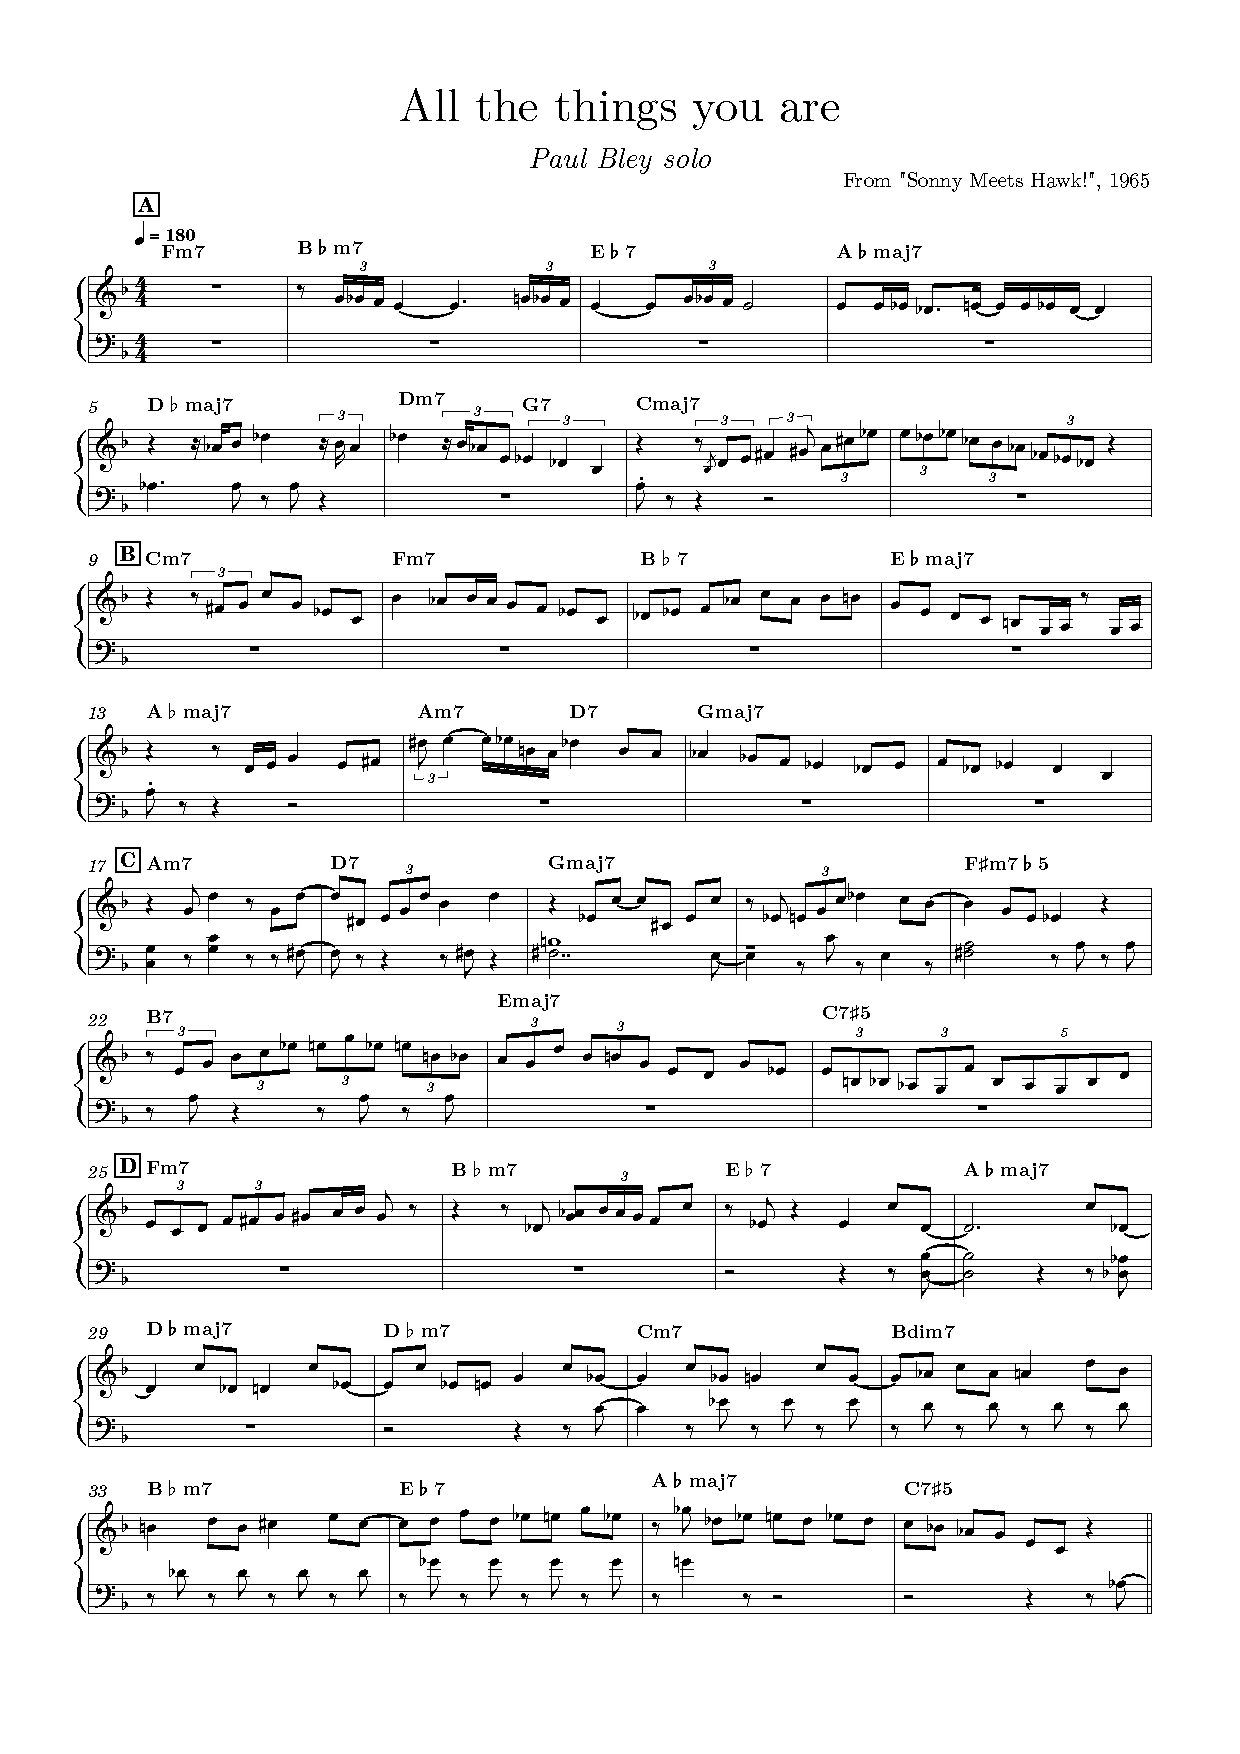
\includepdf[pages=1,pagecommand={\section{All the Things You Are (da \textit{Sonny Meets Hawk!}, 1963)}\label{solo:things}},scale=0.9]{things_vanilla}
\includepdf[pages=2-,pagecommand={},scale=0.9]{things_vanilla}
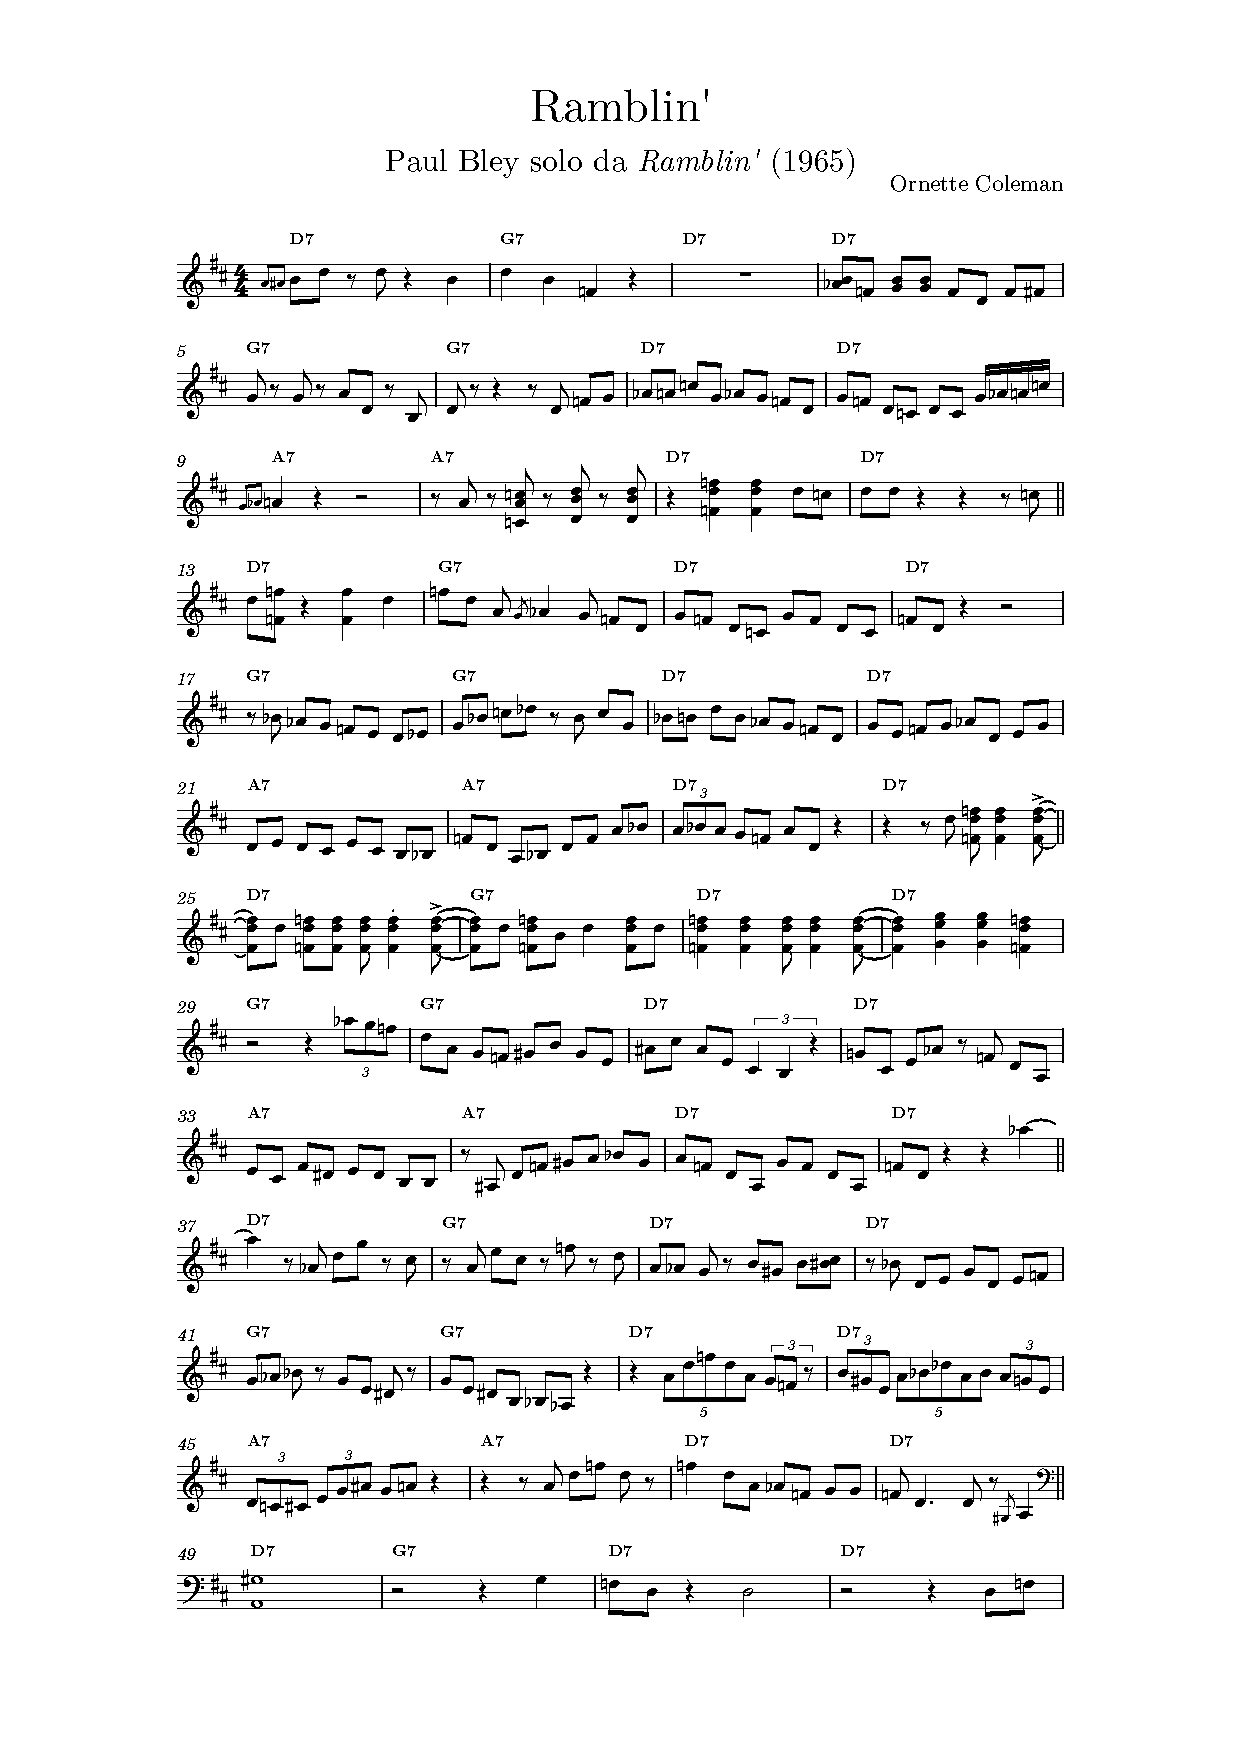
\includepdf[pages=1,pagecommand={\section{Ramblin' (da \textit{Ramblin'}, 1966)}\label{solo:ramblin}},scale=0.9]{ramblin solo vanilla} \includepdf[pages=2-,pagecommand={},scale=0.9]{ramblin solo vanilla}
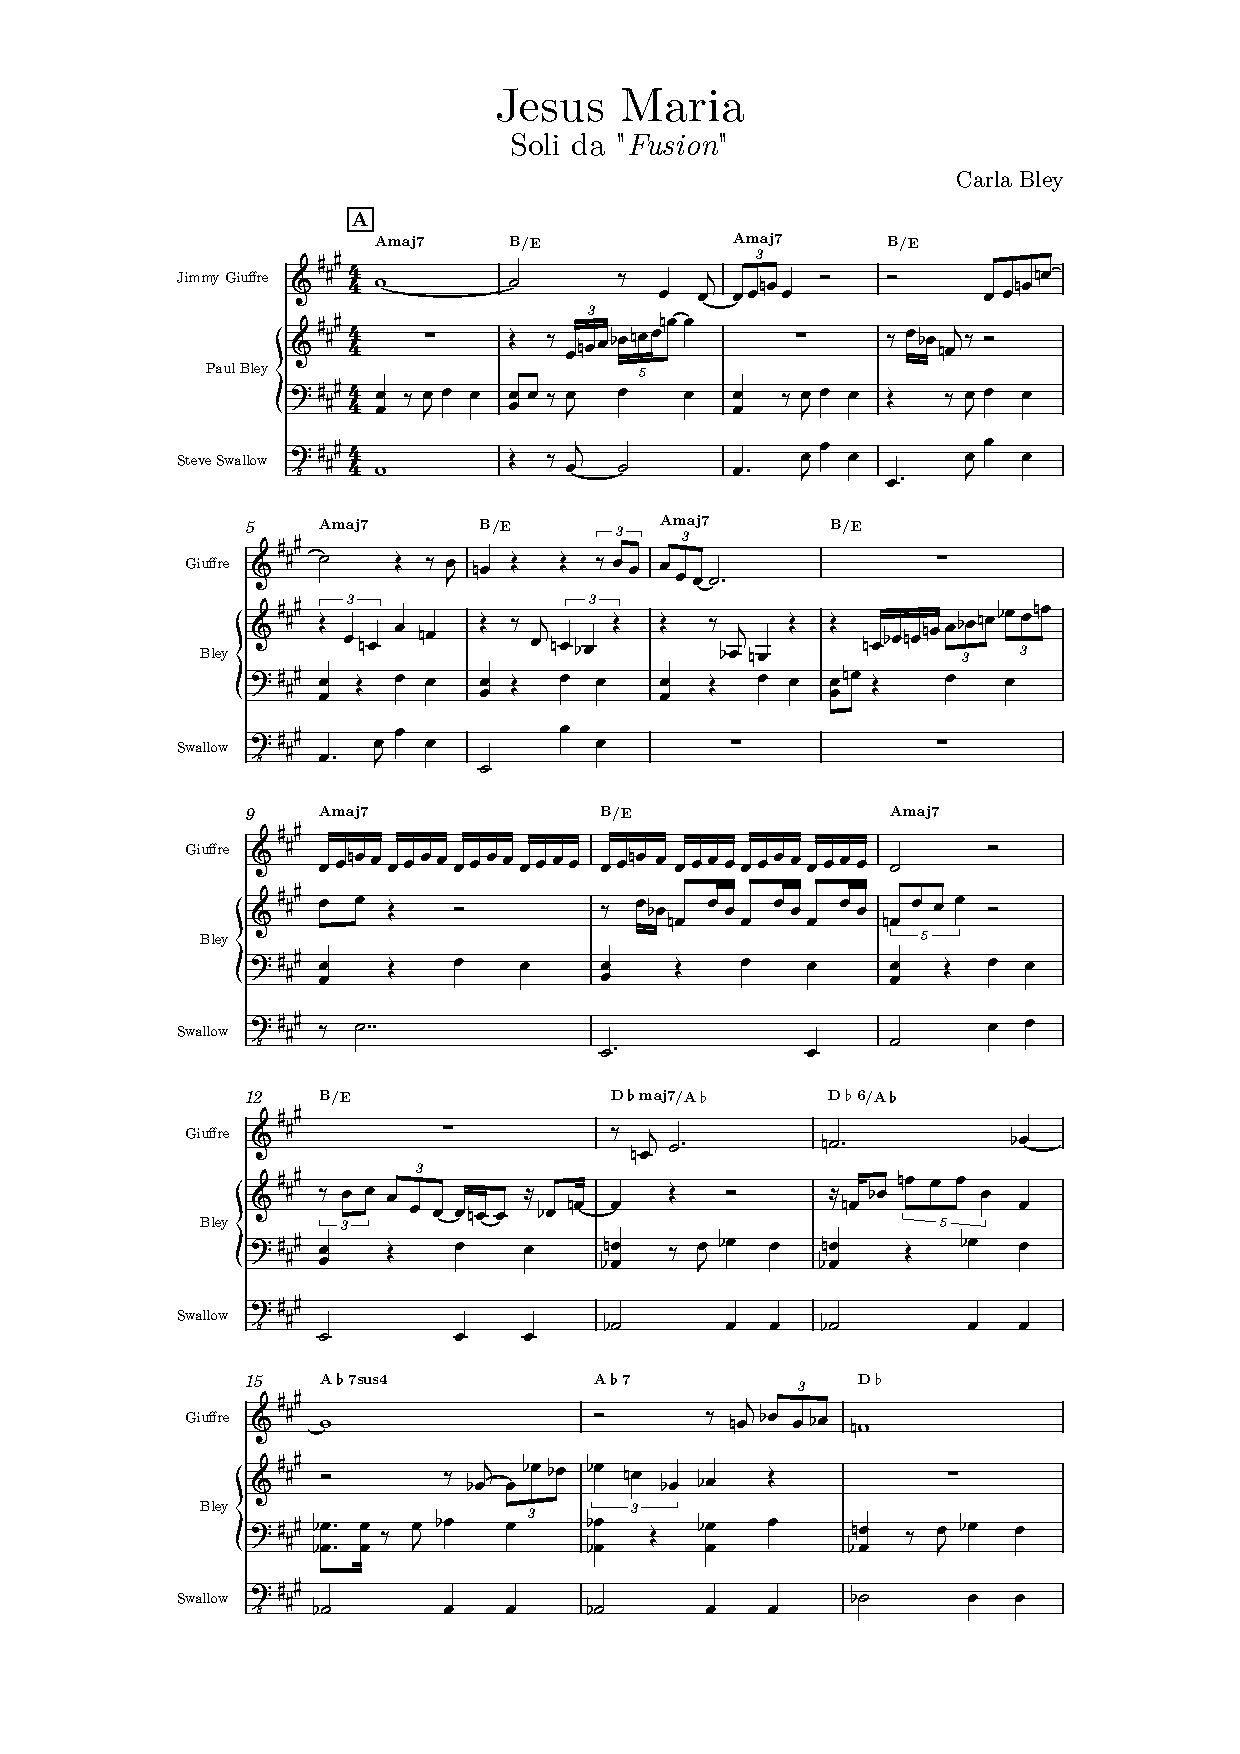
\includepdf[pages=1,pagecommand={\section{Jesus Maria (da \textit{Fusion}, 1961)}\label{solo:jesus}},scale=0.9]{jesus solo}
\includepdf[pages=2-,pagecommand={},scale=0.9]{jesus solo}
\includepdf[pages=1,pagecommand={\section{Ida Lupino (da \textit{Closer}, 1966)}\label{solo:ida}},scale=0.9]{ida_vanilla}
\addcontentsline{toc}{chapter}{Discografia}
\chapter*{Discografia}
\begin{itemize}
	\item Charlie Parker, \textsc{Montreal 1953} [Uptown Records 1993]
	\item Ornette Coleman, \textsc{Ornette Classics 1} [Improvising Artists 1977]
	\item Paul Bley, \textsc{The fabulous Paul Bley quintet} [America Records 1970]
	\item George Russell, \textsc{Jazz in the Space Age} [Decca 1960]
	\item The Jimmy Giuffre 3, \textsc{Fusion} [Verve 1961]
	\item The Jimmy Giuffre 3, \textsc{Thesis} [Verve 1961]
	\item Sonny Rollins \& Coleman Hawkins, \textsc{Sonny meets Hawk!} [RCA Victor 1963]
	\item Paul Bley, \textsc{Turning point}[Improvising Artists 1975]
	\item Paul Bley, \textsc{Barrage} [ESP-disk 1964] 
	\item Paul Bley, \textsc{Closer} [ESP-disk 1965] 
	\item Paul Bley, \textsc{Ramblin'} [RCA Italia 1966]
	\item Paul Bley, \textsc{Improvisie} [America 1971]
	\item Annette \& Paul Bley, \textsc{Dual Unity} [Freedom Records 1972]
	\item Annette Peacock, \textsc{I'm the One'} [RCA 1972]
	\item Paul Bley, \textsc{Open, to Love} [ECM 1972]
	\item Paul Bley \& Niels-Henning Ørsted Pedersen, \textsc{Paul Bley/NHØP} [SteepleChase Records 1973]
	\item Paul Bley, Bill Connors, Jimmy Giuffre, \textsc{Quiet song} [Improvising Artists 1974]
	\item Paul Bley, Steve Swallow \& Jimmy Giuffre, \textsc{The Life of a Trio: Saturday} [Owl Records 1990]
	\item Paul Bley, Steve Swallow \& Jimmy Giuffre, \textsc{The Life of a Trio: Sunday} [Owl Records 1990]
	\item Paul Bley, Steve Swallow \& Jimmy Giuffre, \textsc{Fly away little bird} [Owl Records 1992]
	\item Paul Bley, Steve Swallow \& Jimmy Giuffre, \textsc{Conversations with a Goose} [Soul Note 1996]
\end{itemize}
\end{appendices}
%\listoffigures
